 %
%-----------------------------------------------------------
%% Computer Music Journal LaTeX template
%%
%% September  2009
%% Author: Cornelia Kreutzer, University of Limerick



%---Document preamble
%
\documentclass[letterpaper, 12pt]{article}


\usepackage{cmjStyle} %use CMJ style
\usepackage{natbib} %natbib package, necessary for customized cmj BibTeX style
\bibpunct{(}{)}{;}{a}{}{, } %adapt style of references in text
\doublespacing
\raggedright % use this to remove spacing and hyphenation oddities
\setlength{\parskip}{2ex}
\parindent 24pt
\urlstyle{same} % make url tags have the same font
\setcounter{secnumdepth}{-1} % remove section numbering
\usepackage{epstopdf}
\usepackage{amsmath,amssymb,amsbsy,bm,upgreek,nicefrac}
% \usepackage{todonotes}
\usepackage{microtype}

% Use the Figures subfolder for image files
\graphicspath{{./Figures/}}

%%%%%%%%%%%%%%%%%%% Begin MY PACKAGES %%%%%%%%%%%%%%%%%%%%%
% Uncomment only one of the ones below
\usepackage{anonymize} 		% Uncomment this line to publish
% \usepackage[blind]{anonymize}   %Uncomment this line for blind review

% \usepackage[firstpageonly=true, scale=1, colorspec=0.85]{draftwatermark} % draft watermark

\usepackage{enumitem}           % controls list spacing
\usepackage{longtable}
\usepackage{supertabular}
% \usepackage{pbox}
% \usepackage{caption}          % remove "Table x:" from Appendix
% \usepackage{url}              % hyperlinks 
% \usepackage{hyperref}         % to simplify the use of \href
% \usepackage{subfiles}         % add Appendixes as separate files
% \usepackage{pdfpages}         % include pdf pages for appendices

%=========== Tables ===========
\usepackage{multicol}           % span multiple columns in tables
\usepackage{multirow}           % span multiple rows in tables
\usepackage{tabularx}
\usepackage{tabulary}
\newcolumntype{L}[1]{>{\raggedright\let\newline\\\arraybackslash\hspace{0pt}}m{#1}}
\newcolumntype{C}[1]{>{\centering\let\newline\\\arraybackslash\hspace{0pt}}m{#1}}
\newcolumntype{R}[1]{>{\raggedleft\let\newline\\\arraybackslash\hspace{0pt}}m{#1}}

%%%%%%%%%%%%%%%%%%% End MY PACKAGES %%%%%%%%%%%%%%%%%%%%%


%% ----------------------------------------------------------------------------------------------------------------------------------------
%% CMJ page headers
%% For initial submission use \lhead{Anonymous}
%% On acceptance for publication, use real author surnames for \lhead modeled on the following examples
%%		One author:	\lhead{\small Keislar}
%%		Two authors:	\lhead{\small Keislar and Castine}
%%		Three authors:	\lhead{\small Keislar, Castine, and Rundall}
%%		Four or more:	\lhead{\small Keislar et al.}
%%
\lhead{\small \anonymize{Sullivan, Wanderley and Guastavino}}
% \lhead{\small Sullivan, Wanderley and Guastavino}
% \lhead{\small anonymous}


%% The package endfloat moves all floats (figures, tables...) to the end of the article, as required for the final version of a CMJ article.
%% Leave this package commented out for initial submission, but uncomment it and the following callout commands for the final version. 
% \usepackage{endfloat}
% \renewcommand{\figureplace}{%
%	\begin{center}
%		\textbf{<<TYPE: INSERT \figurename~\thepostfig\ ABOUT HERE.>>}
%	\end{center}}
% \renewcommand{\tableplace}{%
%	\begin{center}
%		\textbf{<<TYPE: INSERT \tablename~\theposttbl\ ABOUT HERE.>>}
%	\end{center}}

%---Document----------
\begin{document}

% {\cmjTitle Design for Performance: From Fiction to Function}
{\cmjTitle From Fiction to Function: Imagining New Instruments Through Design Workshops}
\vspace*{24pt}

% (In the initial submission, omit all the following author information to ensure anonymity during peer review.
% On final submission please make sure that the author address is a complete, functioning postal address.
% Post will be sent to that address.)

% Author: name
{\cmjAuthor \anonymize{John Sullivan, Marcelo Wanderley, and Catherine Guastavino}}	% List all authors here
% {\cmjAuthor author names witheld for anonymity}	% List all authors here
							% e.g.:
							% {\cmjAuthor Doug Keislar, Peter Castine, and Jake Rundall}
 
% Author: address
\begin{cmjAuthorAddress}
    \anonymize{
	Centre for Interdisciplinary Research in Music Media and Technology (CIRMMT), Input Devices and Music Interaction Laboratory (IDMIL), and Multimodal Interaction Laboratory (MIL) \\
	McGill University\\
	527 Sherbrooke St. W. Suite A715 \\
    Montr\'{e}al, QC H3A1E3 Canada \\
	\{john.sullivan2, marcelo.wanderley, catherine.guastavino\}@mcgill.ca}
\end{cmjAuthorAddress}


\begin{abstract}
This paper introduces a set of workshops held with expert musicians to imagine novel musical instruments through design fiction. The workshops were based on the Magic Machine workshops developed by Kristina Andersen, in which participants crafted non-functional prototypes of instruments they would want to use in their own performance practice. Through in-situ activities and post-workshop thematic analysis, a set of design specifications were developed that can be applied to the design of new digital musical instruments intended for use in real-world artistic practice. In addition to generating tangible elements for design, the theories and methods utilized, based in human-computer interaction and human-centered design, are offered as a possible model for merging imaginative idea generation with functional design outputs. 

\end{abstract}

% \section{<<BEGIN ARTICLE>>}

% \section{Introduction}

Digital musical instrument (DMI) design is a broad and interdisciplinary field. Designers engage in the development of new instruments and novel approaches to musical performance (as well as composition and production) for a wide variety of reasons. Even where DMI design is fundamentally research-based, the means and the ends take a variety of forms, ranging from rigorous scientific experimentation to artistically motivated creative practice \citep{Gurevich2016}. Fittingly, the field, and more generally the broad domain of music technology in which it lies, contributes a wide range of outcomes both within and beyond specifically musical applications, such as the development of new technologies for interactive systems \citep{malloch2018generalized} and the advancement of knowledge and theories on technology-mediated artistic performance \citep{Tahlroglu2020}. 

With this work, we were interested to explore a novel method for the design of instruments expressly intended for real-world musical practice. Motivated by previous studies that examined key factors for user engagement \citep{OBrien2008} and longitudinal use of DMIs in performance \citep{Sullivan2019,Wallis2013}, two workshops were held with expert musicians that led to a set of design specifications for the development of new performance instruments. The workshops applied a user-driven approach to the early ideation stages of DMI development through the use of design fiction \citep{Blythe2014} and non-functional prototyping \citep{Pigrem2018} to inspire novel concepts for the new instruments. 

This article is structured as follows. First, we review approaches to, and motivations for, designing novel DMIs. In particular, we consider methods for early stages of ideation and innovation, including user-centered and participatory design approaches drawn from the field of Human-Computer Interaction (HCI) and oriented towards applications for creative practice. We then introduce the Design for Performance workshops, where expert musicians built non-functional prototypes of imaginary DMIs. We present results from the in-workshop activities and thematic analysis of the recorded workshop sessions, and present a set of design specifications. Finally, we discuss the potential efficacy of the design fiction approach towards developing instruments that are viable for uptake and long-term use by expert musicians in real-world performance, and outline future work for robust evaluation of the methods explored.

% We begin with a review of approaches to, and motivations for, designing novel DMIs. In particular, we consider methods for early stages of ideation and innovation, including user-centered and participatory design approaches drawn from HCI and oriented towards applications for creative practice. The Design for Performance workshops are then introduced, where  expert musicians built non-functional prototypes of imaginary DMIs. Section \ref{ch3-sec:results} reports the initial results of the in-workshop activities, and Section \ref{ch3-sec:thematic-analysis} provides the results of the post-workshop analysis that was conducted, which led to the generation of a list of design specifications for new instruments. Finally, Section \ref{ch3-sec:discussion} discusses the potential efficacy of the design fiction approach towards developing instruments that are viable for uptake and long-term use by expert musicians in real-world performance, and outlines future work for robust evaluation of the methods explored. 


\section{Background}
\label{ch3-sec:background}

The ongoing design of new musical instruments is nothing new. However the last 200 years have brought about major changes in why and how new instruments are created. In his book \emph{Sonic Writing}, \citet{Magnusson2019} identifies the nineteenth, twentieth, and twenty-first centuries as rough delineations of three music technological epistemes representing acoustic, electronic, and digital paradigms respectively. Each has defined its own themes for instrument design and related musical practice. 

% The acoustic era is characterized by standardization and reproduction, both in instrument design (as with the industrialization and factory/mass production of the piano and other popular instruments) and practice (in which the prevalent mode of performance was the repetition of written scores). New instruments were most commonly derived from existing instruments \citep{Rubine1990}, often in an effort to address limitations of existing instruments, improve usability, extend functionality or implement better technologies in their design and manufacture \citep{Emerson2018}.

% The electronic era, and later the digital era, ushered in tremendous changes in both design and practice. \citet{Magnusson2019} attributes the transition from acoustic as a shift from symbols (as characterized by individual notes written on a score) to signals, in which sounds and user controls are translated into electronic and digital representations that can be easily and flexibly processed, mapped and mixed. Of course, Magnusson's viewpoint seems to be more focused on the written traditions of classical music, and less towards popular styles which were historically based on oral tradition. Nonetheless, these shifts have largely been brought about by technological advancements irrespective of specific musical traditions. 

% The shift to electronic and then digital introduced the ability to record and play back sound, as well as to synthesize entirely new sounds and manipulate them in many ways. The expanded capabilities of electronic and digital instruments, as well as the wide variety of performance behaviors they afford, is well illustrated by the model of music interaction and performance context developed by \citet{Malloch2006} shown in Figure \ref{ch3-fig:malloch-model-of-interaction}. Adapted from Rasmussen's model of human information processing \citep*{Rasmussen1986}, the figure illustrates a continuum of performance behaviors and contexts from right to left, moving from conventional instruments (consisting of note-level, real-time, skill-based interactions that would be typical of acoustic playing) to novel performance modes and instruments that are rule- and model-based in operation, made possible by advanced electronic and digital technologies for signal processing, sampling, synthesis, mixing, mapping and more.

% \begin{figure}[htpb]
%     \centering
%     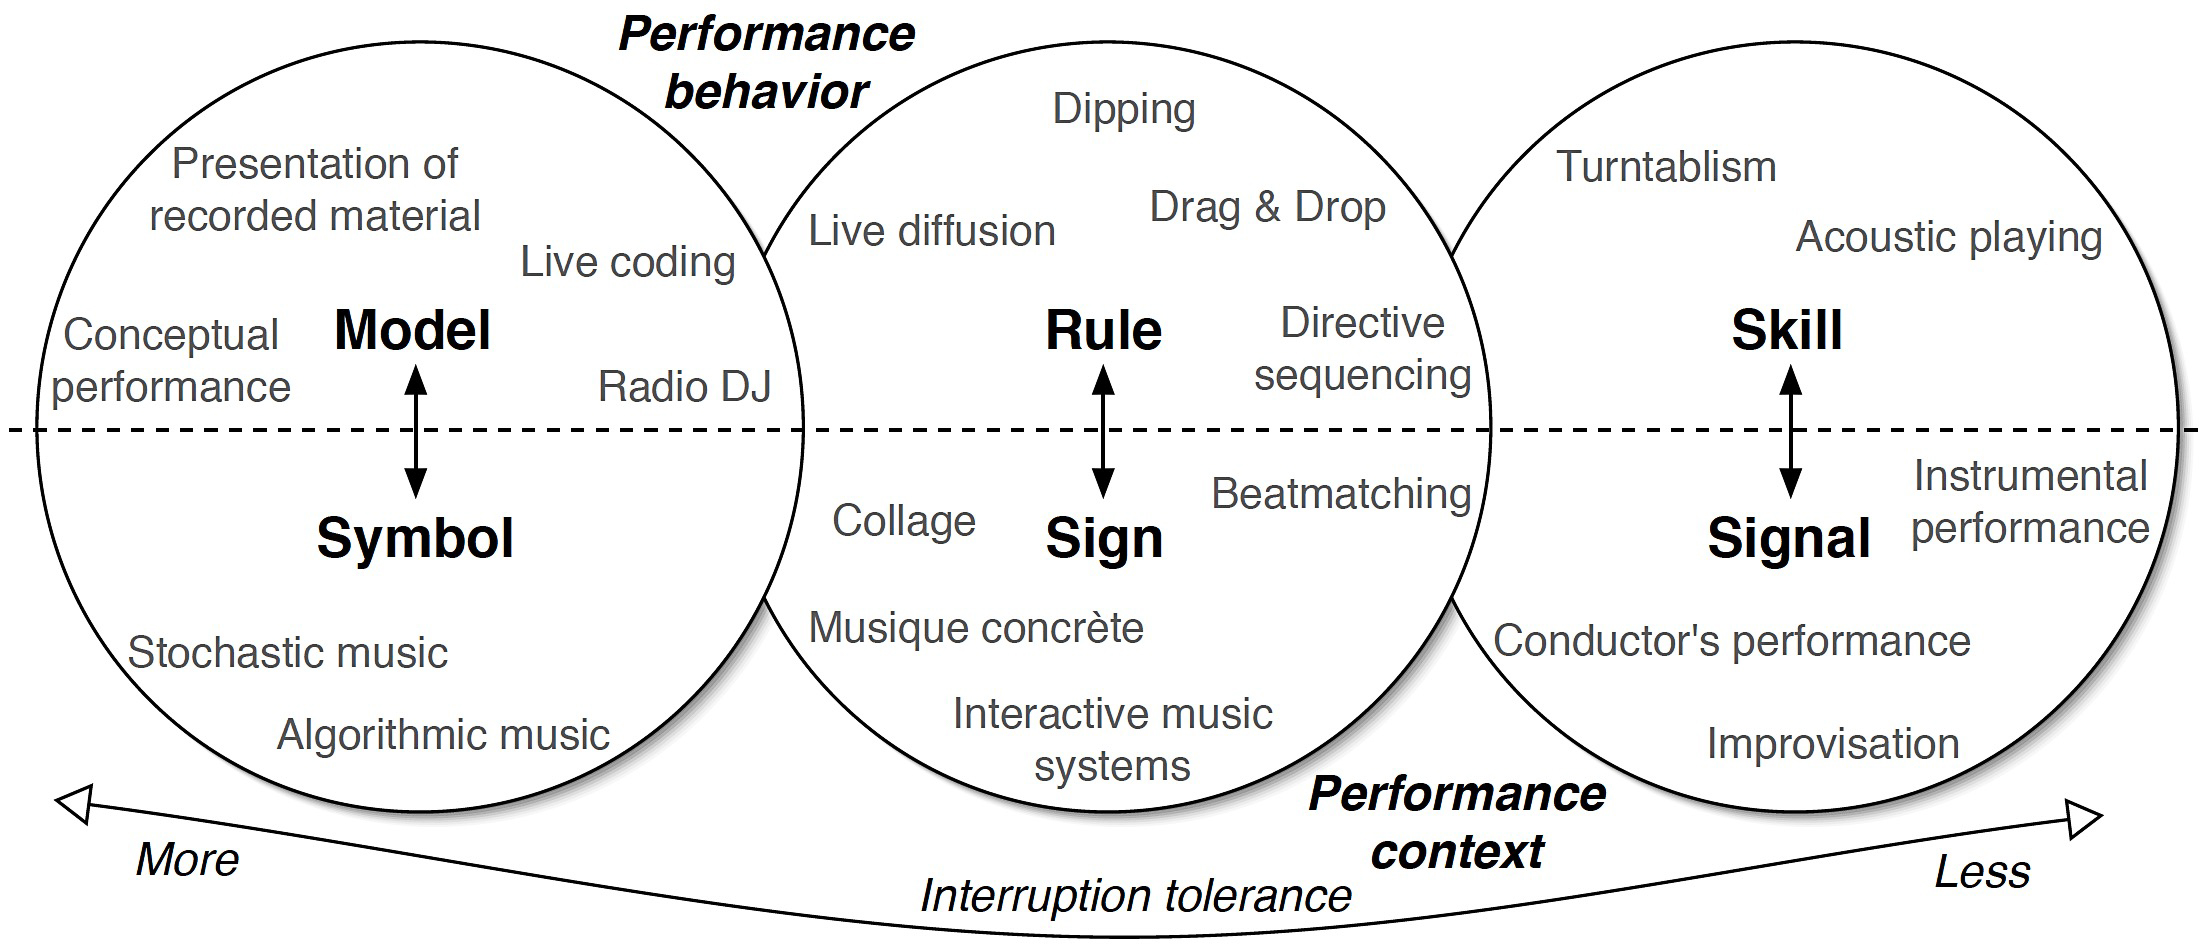
\includegraphics[width=0.83\textwidth]{ch3_malloch_model_of_interaction.jpg}
%     \caption[Model of music interaction and performance contexts]{Model of music interaction and performance contexts by \citet{Malloch2006}. Note that \emph{symbol} and \emph{signal} are defined here by the figure's authors and unrelated to the terms as used by \citet{Magnusson2019}.}
%     \label{ch3-fig:malloch-model-of-interaction}
% \end{figure}

An important aspect of the progression from acoustic to electronic, then digital instruments has been the decoupling of the user input from sound production. An instrument's sound is typically generated and controlled through the various performative actions of its owner.
% (There are, of course, exceptions to this model, especially in the digital domain, such as instruments that behave autonomously or receive input from arbitrary input data, which are outside of our scope of consideration.)
On an acoustic instrument these sound-producing actions, or \emph{instrumental gestures} \citep{Cadoz1988}, are physically and mechanically linked to a sonic result. On the other hand, a digital instrument is not driven by acoustic means and the link between control and sound occurs in the digital realm. Thus, the designer is free to choose any type of input control and any system of mapping controls to sound. From the designer's perspective this ultimate freedom may be liberating, and is reflected in the increasing quantity, complexity and diversity of new DMIs that have been developed over the last few decades. However this may also present a challenge for designers. Magnusson characterizes the digital era as one in which ``any bodily gesture can be mapped to any sound and there is no natural paradigm at play that we can relate to'' \citep*[p. 34]{Magnusson2019}. While the issue of mapping is a deep area of research and scholarship in its own right (see \citet{os-mapping-2002} and \citet{cmj-mapping-2014} for in-depth reports), here we focus on two more basic inquiries: First, if few technical and conceptual limitations exist, what motivates the design of new DMIs? And second, what methods are effective in the development of novel DMIs that will make them appealing for use in artistic practice?

\subsection{Diverse motivations for designing new instruments}
\label{ch3-sec:diverse-motivations-for-designing-new-instruments}

There are a wide range of factors that motivate the design of DMIs. In research settings, it may be useful to design DMIs that are specific to a particular experimental context \citep{Marquez-borbon2011}. A survey by \citet{Morreale2017} of DMI designers presenting instruments at the International Conference on New Interfaces for Musical Expression (NIME) found this to be a common approach: out of the 97 instruments included in the study, 38 (39\%) were reported to have been designed as research probes. In these circumstances, the instruments' actual use in real-world performance may be of secondary importance to more immediate research objectives. When considering performance with new instruments in more widespread contexts, social, cultural and economic factors come into play, in particular market and consumer-driven behaviors that influence trends, popularity and visibility of commercial, off-the-shelf instruments \citep{Theberge1997}. The diversity of design approaches and objectives (in particular between commercial and research-based designs) has been highlighted by \citet{mcpherson2019musical} in a comparison of instruments emerging from different domains including NIME, HCI, and crowdfunding campaigns. 

A study by \citet{Emerson2018} that focused specifically on the design of DMIs expressly intended for artistic practice identified four primary categories of motivation: facilitating greater embodiment in performance, improving audience experience, developing new sounds, and building responsive systems for improvisation. They also highlighted different motivations based on the context of participants' practices: those more active in academic settings exhibited more interest new sounds and responsive systems for improvisation, while others who performed in club settings were motivated to improve embodiment and audience experience.

\subsection{DMI design and HCI}
\label{ch3-sec:dmi-design-and-hci}

The diverse motivations for designing new instruments are also reflected in various design approaches and methodologies used. Much of the prevailing discourse on DMI design comes from the field of HCI, which over time has evolved from quantitative and rigid strategies \citep{Bodker2015} to paradigms that are better suited to accommodate idiosyncratic approaches that are frequently found in music interaction contexts \citep{Wanderley2002}. Second wave HCI emerged to include perspectives on technology within social, cultural and organizational contexts \citep{kaptelinin2003}, with an emphasis on user-centered, qualitative methods theoretically grounded in situated action, distributed cognition and activity theory \citep{Bodker2006}. The third wave has continued to expand the purview of HCI to accommodate the ubiquitous nature of technology, prioritizing experiences, meaning-making and emergent use \citep{Bodker2015}. This third paradigm is phenomenologically situated with a focus on embodied interaction, that can embrace multiple interpretations and yield rich understandings supported by ethnographic and practice-based research approaches \citep{Bodker2015}. The third paradigm of HCI is characterized by \citet{Harrison2007}.

% The diverse motivations for designing new instruments are also reflected in various design approaches and methodologies used. Much of the prevailing discourse on DMI design research comes from the field of HCI, which can provide prescriptive strategies for for all stages of the design process. Early HCI favored systematic approaches, rigid guidelines and formal methods for designing and evaluating human-machine interfaces \citep{Bodker2015}. Examples in DMI research include the formulation of quantitative methodologies like Fitts's Law and Meyer's Law to evaluate target acquisition in the context of musical interactions \citet{Wanderley2002}, and schema developed by \citet{Vertegaal1996c} to match transducers and feedback modes to specific musical functions. However, limitations to these methods have been highlighted in the design of music interactions, which are often characterized by idiosyncratic approaches, driven by ``precise artistic demands'' \citep*[p. 67]{Wanderley2002} to yield highly creative and innovative results.

% HCI has also evolved to provide more nuanced approaches to design research. Second wave HCI emerged to include perspectives on technology within social, cultural and organizational contexts \citep{kaptelinin2003}, with an emphasis on user-centered, qualitative methods theoretically grounded in situated action, distributed cognition and activity theory \citep{Bodker2006}. The third wave expanded the purview of HCI to accommodate the ubiquitous nature of technology, prioritizing experiences, meaning-making and emergent use \citep{Bodker2015}. The third paradigm of HCI is characterized by \citet{Harrison2007} as phenomenologically situated with a focus on embodied interaction, that can embrace multiple interpretations and yield rich understandings supported by ethnographic and practice-based research approaches.

\subsubsection{User-centered, human-centered and participatory design}
\label{ch3-sec:user-centered-design}


User-centered design (UCD) is a common approach within HCI where users are systematically involved throughout the design process. \citet{Norman1988} popularized the term, in which the designer should ``ask what the goals and needs of the users are, what tools they need, what kinds of tasks they wish to perform, and what methods they prefer to use'' \citep[as cited in][p. 44]{El-shimy2014}. UCD is less of a method in and of itself than a high level guideline under which several design strategies fall such as those in \citet{greenberg2011sketching}. 
% Attitudes towards UCD have evolved over time and, while UCD is still widely used in practice and reference, human-centered design (HCD) has emerged as a subtle but important variation. \citet{Norman2013} describes HCD as a design philosophy and set of procedures that are complementary to more specific areas of focus such as experience design, industrial design and interaction design.
% \footnote{HCD is also formally defined as an ISO (International Organization for Standardization) standard, however UCD is not.} 
% that add ``deep consideration and study of human needs to the design process, whatever the product or server, whatever the focus'' \citep*[p. 10]{Norman2013}. The \emph{human}-centered scope of HCD provides a the opportunity for wider consideration and different contexts of people in product and interaction design, instead of ``a narrower focus on peoples roles as \emph{users}'' \citep[p. 45]{Steen2011}.
% Human-centered design (HCD) \citep*{Norman2013} has evolved from UCD
% UCD is less of a method in and of itself than a high level guideline under which several design approaches fall. Human-centered design (HCD) is a second term popularized by Norman in \citep*{Norman2013}. 
Human-centered design (HCD) has emerged as a subtle but important variation \citep{Norman2013}, allowing for a broader consideration of people with regards to design, instead of ``a narrower focus on peoples roles as \emph{users}'' \citep[p. 45]{Steen2011}. This corresponds with trends in HCI: ``Instead of focusing on how specific tools can be designed to help users accomplish specific tasks, the human-centered perspective encourages developers to strive for a better understanding of how people live in the world, and to design systems accordingly'' \citep[p. 45]{El-shimy2014}. 

Participatory design (PD) is an HCD approach that became well-established with second-wave HCI \citep{Bodker2015} and has continued to be relevant in third-wave HCI as well \citep{Muller2012}. It is predicated on the full participation of end-users through all stages of the design process \citep{Steen2011}, and is primarily concerned with the \emph{tacit knowledge} of the involved participants which, according to \citet{Spinuzzi2005}, is hard to formalize and had been missing from early HCI. In DMI research, PD methods have been applied in the design and evaluation of Theremin-based controllers \citep{Geiger2008}, audio-haptic interfaces for the visually impaired \citep{Metatla2016}, and more generally to investigate music interaction design based on conceptual metaphor theory \citep{wilkie2013towards} and digital musical interaction ecologies \citep{Fyans:2012}.

It is important to note that the roots of PD are also political, and it was originally envisioned as a way ``to rebalance power and agency among managers and workers'' \citep[p. 1]{Bannon2018}. Some current PD practices have been critiqued as merely UCD by a different name, lacking the original political and activist contexts \citep{Bannon2018}. Our own work presented here uses methods that fall under the PD umbrella but without any specific political motivation; therefore we identify our approach as HCD and refrain from characterizing it as full PD in deference to these objections.

% \begin{quote}
%     It is a far cry from earlier work in the field, where Participatory Design not only sought to incorporate users in design, but also to intervene upon situations of conflict through developing more democratic processes. \citep[p. 2]{Bannon2018}. 
% \end{quote}

% We note that our own work presented here uses HCD methods that fall under the PD umbrella but without any specific political motivation; therefore we present our approach as HCD and refrain from characterizing it as full PD in deference to these aforementioned objections raised by \citeauthor{Bannon2018}. 


\subsubsection{Design frameworks}
\label{ch3-sec:design-frameworks}

Many different frameworks have been developed for the design and evaluation of new DMIs. Earlier examples include models based on categories of musical interaction \citep{Bongers2000a}, structural components of DMIs \citep{Wanderley2004}, addressing diverse needs of different performers \citep{Jorda2004, Jorda2004b}, interdisciplinary approaches combining music performance, HCI and digital technology \citep{Overholt2009}, and user experience tracking \citep{fmorreale:2014}. Evaluation frameworks include include those based on the roles of various stakeholders \citep{OModhrain2011a} and formal HCI techniques \citep{Young2015a}.

\subsection{Novel approaches to idea generation and prototyping}
\label{ch3-sec:novel-approaches-to-idea-generation-and-prototyping}

While high level design frameworks may be helpful in formulating a conceptual approach, they are generally not oriented towards specific design tools and methods. For our own work, we wish to develop effective strategies for developing new instruments that will be appealing for musicians to incorporate into their real-world creative practice. In particular, we look at two user-driven approaches to generating ideas for new designs: a physical DMI prototyping toolkit and a design workshop methodology. 

\subsubsection{Probatio}
\label{ch3-sec:probatio}

Probatio is a system developed by \citet{Calegario2019} that is comprised of a set of physical modules and accompanying methodology for exploring ideas and developing proof-of-concept DMI prototypes. It is meant to address a few important issues that arise in DMI design: for one, it provides functional constraints to limit the endless possibilities and increased complexity that arises from the separated user input and sound production components of DMIs, which can lead to ``creative paralysis'' \citep{Magnusson2010}. For another, it can help speed up and eliminate bottlenecks for iterative design, facilitating rapid design and evaluation cycles. The Probatio hardware consists of several control blocks, each featuring a different type of input control (ie., buttons, slider, crank, etc.), and different bases and structural supports that can accommodate variable configurations of the control blocks. The hardware is engineered so that the blocks attach magnetically and electrical connections are made automatically. Control signals are then mapped to sound synthesis software, making the prototype instantly playable as soon as one or more blocks are connected. An example Probatio prototype is shown in Figure \ref{ch3-fig:probatio-assembly}.

\begin{figure}[htbp]
    \centering
    \begin{subfigure}[t]{0.485\textwidth}
        \centering
        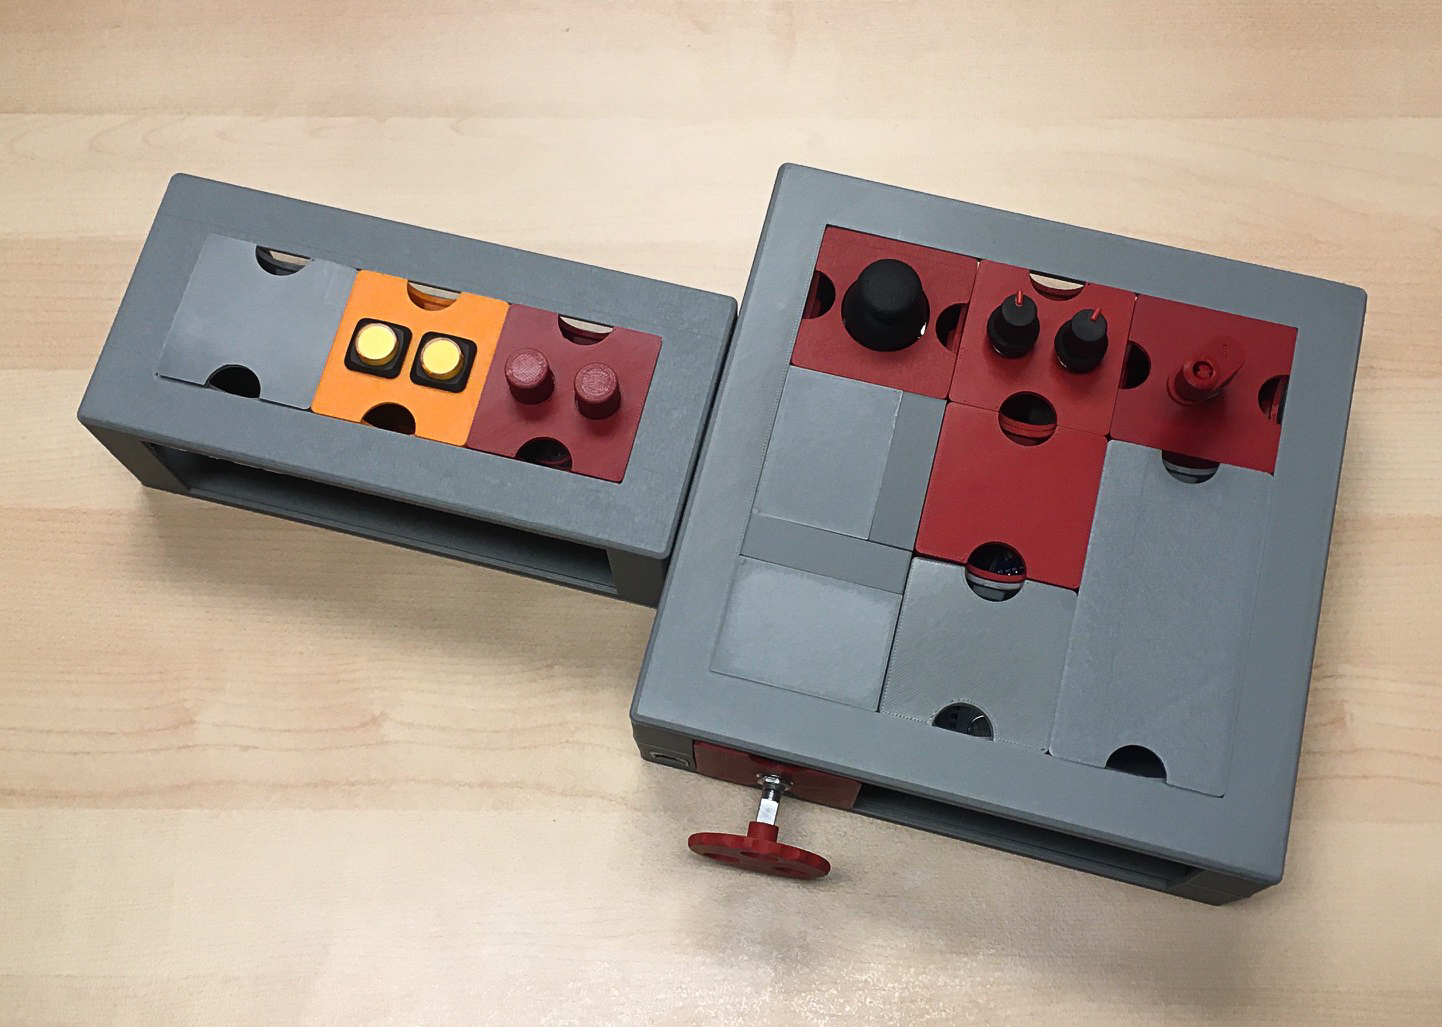
\includegraphics[width=1\textwidth]{ch3_probatio_assembly.jpg}
        \caption[]{A prototype constructed with a Probatio base, structural support and several control modules.}
        \label{ch3-fig:probatio-assembly}
    \end{subfigure}
    ~
    \begin{subfigure}[t]{0.485\textwidth}
        \centering
        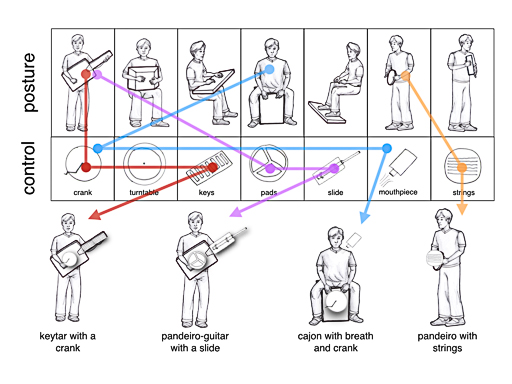
\includegraphics[width=1\textwidth]{ch3_probatio_chart.jpg}
        \caption{Morphological chart suggesting new prototypes by combining features of existing instruments. Drawings by Giordano Cabral.}
        \label{ch3-fig:probatio-chart}
    \end{subfigure}
    \caption[The Probatio toolkit.]{The Probatio toolkit, version 1.0, by \citet{Calegario2020}.}
\end{figure}

The methods that guide the use of the Probatio toolkit are based on Calegario's concept of \emph{instrumental inheritance} in which aspects of existing instruments such as physical structures, playing techniques and specific types of input controls can be explored in different combinations and configurations, yielding entirely new instruments. A morphological chart \citep{Cross2000}, shown in Figure \ref{ch3-fig:probatio-chart}, assists the designer in this process, presenting different postures and controls that can be constructed with the Probatio hardware.

\subsubsection{Magic machines and design fiction}

Another compelling approach to idea generation and prototyping for DMI design comes with ``Magic Machine'' workshops developed by \citet{Andersen2017}. The workshops ``make use of the notion of technology as a `magical unknown' as the starting point for a range of workshop techniques that begin with material exploration'' \citep[p. 4971]{Blythe2016}. In them, participants are prompted to make non-functional low-fi prototypes out of generic crafting materials like cardboard, wood, string, and glue. Once finished, they present their creations, demonstrating their use in imagined scenarios.

The Magic Machine workshops have some basis in design fiction, where concepts and problems can be explored through the development of imaginary scenarios and ``fantasy prototypes'' \citep{Sterling2009}. Importantly, the artefacts that are generated (the non-functional prototypes) are not overly meaningful in and of themselves, and the ultimate aim is not solve any given problem. Rather, the processes of creating and engaging with the ``magical unknown'' serves ``to give temporary body to concerns and questions [and] to consider the potential reality of a world in which such a thing might exist'' \citep[p. 4971]{Blythe2016}.

Andersen has run the workshops is a variety of of contexts for both adults and children, including workshops for the design of new (imagined) musical instruments. The workshop was also utilized by \citet{Lepri2019} in a study that explored diverse values and priorities of different music cultures, backgrounds and contexts.

\subsubsection{Towards design for performance}
\label{towards-design-for-performance}

The Probatio toolkit and Magic Machine workshops present dynamic methods for early ideation stages of DMI design that we are interested in applying to our own work. The workshops offer a creative approach for generating ideas free from technological or practical constraints, while Probatio provides a clearly defined set of tools to quickly construct and evaluate prototypes. The next section reports on our own workshop that was styled after the Magic Machines workshop.
% It includes additional details about Andersen's methods and our own customizations to orient the activities to address our specific goals and inquiries. 
In the discussion that follows we consider how our own methodology can be complementary to the well-structured Probatio approach to ideation and functional prototyping, and if and where the two can overlap. 

\section{The Design for Performance workshop}
\label{ch3-sec:design-for-performance-workshop}

The Design for Performance workshop was developed to involve expert musicians in the early stage ideation of new instruments, and draws from a variety of general methods from HCD and PD that have been mentioned so far: design workshops, non-functional and low-fidelity prototyping, and design fiction. 
% In this section we introduce the Design for Performance workshop, where expert musicians envisioned and crafted fictional musical instruments. The structure draws from a variety of general methods from UCD and PD that have been mentioned so far: design workshops, non-functional and low-fidelity prototyping, iterative design, and design fiction. The workshop is envisioned as part of a multi-stage design study, with additional phases of the project to follow (See Chapter \ref{ch4-cha} for the workshop results applied in the design of new DMIs, and Section \ref{ch3-sec:limitations-and-future-work} for a discussion on current limitations and future work.)
The structure is based on Andersen's Magic Machine workshops but is revised to direct the outcomes towards the generation of design specifications that could be applied to the development of new performance-ready DMIs. 
% Table \ref{ch3-tab:workshop-activities} provides a side by side comparison of the the Design for Performance and Magic Machine workshop activities (in particular Andersen's musical instrument design workshops \citep*[pp. 30-53]{Andersen2017}) and notes variations between them. In Section \ref{ch3-sec:workshop-activities} we describe each activity in detail.

% \begin{table}[thbp]
%     \footnotesize
%     \begin{center}
%         \begin{tabular}{ l c c L{5cm} L{5cm} }
% 			% % \hline % \toprule
% \hline
% 			\hline
%             \textbf{Activity} &
%             \textbf{DP} &
%             \textbf{MM} &
%             \textbf{Description} &
%             \textbf{Variations} \\
% 			% % \hline % \midrule
% \hline
% 			\hline
%             Introduction & X & X 
%             & Introduce workshop and set out rules 
%             & \\ 
%             \hline
%             Prompt & X & X 
%             & Draw the imagined sound/music you wish to create.
%             & MM: The prompt is drawn in permanent marker on hand. DP: Prompt is drawn on index card. \\
%             \hline
%             Build & X & X 
%             & Create non-functional instrument prototypes from provided crafting materials
%             & \\
%             \hline
%             Present & X & X 
%             & Each participant presents their instrument with demonstration and explanation.
%             & DP: During presentations, the facilitator takes note of defining elements of the instrument and adds them to a whiteboard underneath category headings. \\
%             \hline
%             Discuss (1) & X & X
%             & A short discussion follows each presentation to explore the instrument and its design.
%             & DP: Presenter and other participants suggest additional elements to be added to the whiteboard. \\
%             \hline
%             Evaluate & X &  
%             & Participants dot-vote the elements they find most compelling in the design of a new instrument. 
%             & DP only. \\
%             \hline
%             Discuss (2) & X &  
%             & A group discussion discussion is held to reflect on voted elements and the prospects for their application in design. 
%             & DP only. \\
%             \hline
%             Document & & X 
%             & Each instrument is photographed and documented.
%             & MM only. (In DP, photographs are taken during presentations.) \\
% 			% % \hline % \bottomrule
% \hline
% 			\hline
%         \end{tabular}
%     \end{center}
%     \caption[Design for Performance and Magic Machine workshop activities]{Comparison of activities for the Design for Performance (DP) and Magic Machine (MM) workshops, noting any significant differences between the activities.}
%     \label{ch3-tab:workshop-activities}
% \end{table}

The context of the Design for Performance workshops marks an important shift from Andersen's Magic Machine workshops, which are specifically oriented towards building diverse design knowledge and complex understandings ``about technology, rather than of technology'' \citep[p. 1]{Andersen2019}. Our approach seeks to find a middle ground between theoretical knowledge and functional design, connecting the diversity and creative freedom fostered by the Magic Machine activities with a holistic design ecology from ideation to finished product. In this way, the Design for Performance workshop is envisioned as a design tool that can elicit preliminary ideas from a group of expert practitioners and translate them into tangible elements that designers can work with. This may be especially valuable in the DMI design space, where idiosyncratic approaches and highly personalized designs are common, and widespread adoption of new DMIs is limited.

% A detailed schedule and script (included in Appendix \ref{axC-sec:schedule-and-script}) was drafted based on Andersen's recommendations to run the workshop at a quick pace and keep a tight timeline. This was found to be an effective strategy to alleviate any potential anxieties or fears of failure that participants could experience during the creative and open-ended design activities \citep{Andersen2017}.

\subsection{Crafting materials}
\label{ch3-sec:crafting-materials}

The main activity of the workshop is for participants to design fictional musical instruments out of provided materials, and the type of materials used can have a large impact on the outcomes of the workshop. Through several incarnations of the Magic Machine workshops (that have utilized an array of different crafting materials, from wood and paper to gumdrops) \citet{Andersen2019} provides recommendations and rationales for the selection of materials. Importantly, generic and potentially absurd or impractical qualities of the materials chosen are essential to the activity. In being tasked with building something concrete out of ill-suited materials, the participant is freed from working within practical constraints or following known traditional methods. Furthermore, Andersen emphasizes that any material has the potential to influence the design outcome: particular objects or shapes may suggest typical or obvious uses, which should be avoided. 

In the case of musical instrument design, materials may have sound-producing properties that a participant may want to apply in their design. However, Andersen specifies that materials should not be utilized for their acoustic qualities. In this way, the prototypes are explicitly \emph{non-functional} and the design activity is oriented towards the imagining of abstract features and novel forms without concern for feasibility or technical implementation. 

For the Design for Performance workshop, we selected a wide range of basic crafting and stationary items purchased from a dollar store, including paper, posterboard, colored index cards and sticky notes, rubber bands, string, wire, popsicle sticks, paper plates, cups, tape, and glue. 
% As our goals differed from those of the Magic Machine workshops and we were interested in in tangible design outcomes, we were open to more conventional designs and included some items that might be predictable in their use. For example, each participant was given a large posterboard from which structural shapes could be fashioned, while index cards, colored tape and magic markers would make it easy for participants to draw in graphical user interfaces (GUIs) and other features typical of DMIs.

% For the Design for Performance workshop, we selected a wide range of basic items purchased from a dollar store. Materials included:

% \begin{multicols}{4}
%     \begin{itemize}[noitemsep]
%         \item posterboard
%         \item index cards
%         \item sticky notes
%         \item string
%         \item wire
%         \item rubber bands
%         \item popsicle sticks
%         \item plastic mesh
%         \item paper plates
%         \item plastic cups
%         \item magic markers
%         \item tape
%         \item glue
%         \item paper clips
%         \item scissors
%         \item utility knives
%     \end{itemize}
% \end{multicols}

\subsection{Pilot}
\label{ch3-sec:pilot}

Prior to the official sessions, a pilot test was carried out to run the full workshop from start to finish. Six master's students who were enrolled in a seminar about musical interface design participated. The session was facilitated by the first author who was assisted by another master's student.
% \footnote{The assistant, Collin Wang, was a master's student supervised by the last author.} 
The session was observed by two colleagues of the facilitator (a music technology Ph.D. student and visiting professor). After the session an informal discussion was held with the participants and observers to get feedback and take suggestions for any improvements that could be made. All generally agreed on the activities and format, while details for minor changes were noted and incorporated into the final structure.  

While not a focus of this specific study, an interesting contrast between the pilot and official sessions is noted in that the pilot participants were all well-versed in DMI design research. On the other hand, the participants who took part in the official workshops were selected for their experience as active performing musicians and not required to have any preexisting knowledge of DMI design (though some did have some design experience too). As the pilot study was constructed to test and rehearse the workshop design, and not for data collection and analysis, no further investigation was made around this at the present. However, it suggests a compelling direction to explore for future workshops, and we can envision potentially different outcomes between designers and non-designers. 

\subsection{Participant selection and consent}
\label{ch3-sec:participant-criteria-and-selection}

% \subsubsection{Research ethics and participant consent}
% \label{ch3-sec:research-ethics-and-participant-consent}

% Before recruitment began, the Design for Performance workshop was reviewed and approved by the Research Ethics Board Office of McGill University (certificate included in Appendix \ref{axD:reb-ethics-certificates}). This approval requires that studies involving human participants follow specific guidelines for research ethics, to ensure safe handling of data and participants' right to privacy and informed consent. While the participants' names, personal information and gathered data would be anonymized, the proceedings would be photographed and video and audio recorded for later analysis and documentation. Participants would be asked permission to use their likenesses (photos, videos or audio) to be used in public disseminations, including this report. Individuals choosing to opt out would still be welcome to participate fully in the workshop and with their recorded presence removed from any publicized documentation.

\subsubsection{Criteria and recruitment}
\label{ch3-sec:criteria-and-recruitment}

As the workshop was focused on the design of DMIs for use in live performance and intended to be held with expert musicians, we identified three main criteria for prospective participants:

\begin{enumerate}[noitemsep]
    \item They should use, or at least be familiar with, digital, electronic or computer-based instruments for musical performance.
    \item They should maintain an active practice, performing in public on a regular basis (at least five times per year). 
    \item Their performance practice should be related to electronic, electro-acoustic or other musical styles in which DMIs are typically used.
\end{enumerate}

A call for participation was circulated through local academic and performance community mailing lists that were likely to reach individuals matching our criteria. 
% \begin{itemize}[noitemsep]
%     \item McGill University Music Technology Area Graduate Students
%     \item Université de Montréal Music Faculty Students
%     \item Centre for Interdisciplinary Research in Music Media and Technology (CIRMMT)
%     %\footnote{\url{https://www.cirmmt.org}} 
%     Members and Students
%     \item Eastern Bloc New Media and Production Centre 
%     \footnote{\url{https://easternbloc.ca}}
%     \item Montréal Contemporary Music Lab\footnote{\url{https://www.labomontreal.com}}
% \end{itemize}
Interested parties were invited to complete an online prescreening questionnaire. Recruitment lasted for two weeks and 25 responses were received. Fifteen individuals who met the criteria were invited to participate, divided into two sessions. Five declined or did not respond, leaving a total of ten participants. To accommodate schedules, the workshop was divided into two sessions, with three participants in session A and seven in the session B. Profiles of each participant are included in Appendix 1.

The Design for Performance workshop was reviewed and approved by the Research Ethics Board Office of \anonymize{McGill University} to ensure that all applicable guidelines were followed for research ethics, safe handling of data, and participants' right to privacy. Before the start of the workshop participants were asked to read and sign an information and consent form that outlined how the workshop would run and explained their rights as participants. Permission was requested for video and audio recording the sessions, as well as for taking photos, to which all participants agreed.

\subsection{Workshop activities}
\label{ch3-sec:workshop-activities}

A schedule for the workshop had been developed based on Andersen's recommendations to run the workshop at a quick pace and keep a tight timeline. This was found to be an effective strategy to alleviate any potential anxieties or fears of failure that participants could experience during the creative and open-ended design activities \citep{Andersen2017}. The sessions were held on consecutive days in a spacious and well lit conference room at the \anonymize{Centre for Interdisciplinary Research in Music Media and Technology (CIRMMT) at McGill Universtity}. Tables were arranged together so that participants sat around the outside facing each other. Crafting materials were arranged on a separate table and covered with a cloth when the participants arrived. 

The first author acted as the facilitator and was aided by the same assistant from the pilot session. Each session began with a welcome and introduction by the facilitator, then participants were asked to briefly introduced themselves and give a short summary of their musical practice and experience with DMIs. 

% \subsubsection{Introduction}
% \label{ch3-sec:introduction}

% Before starting the workshop activities participants were asked to read and sign an information and consent form that outlined how the workshop would run and explained their rights as participants. Permission was requested for video and audio recording the sessions, as well as for taking photos, to which all participants agreed.

% Each session began with a welcome and introduction by the facilitator. Participants were asked to briefly introduced themselves and give a short summary of their musical practice, as well as any interest or experience they had in instrument design. 

% The workshop began with the facilitator introducing themselves and the assistant, and giving additional context and background about the workshop and related research. Then participants went around the room and introduced themselves and gave a short summary of their musical practice, as well as any interest or experience they had in instrument design. Finally, the facilitator presented five guidelines to establish the intended mood for the ensuing activities: 

% \begin{enumerate}[noitemsep]
%     \item There is no right or wrong.
%     \item The activities are short, so move quickly.
%     \item Be honest, respectful, and supportive to yourself and the other participants. 
%     \item Make sure everybody can be heard. 
%     \item Be creative, enjoy the process and have fun with it!
% \end{enumerate}

\subsubsection{Activity 1: Prompt}
\label{ch3-sec:activity-1-prompt}

The workshop activities began with a prompt. Participants were asked to think of the music that currently make or would like to make, and then instructed to ``draw the music'' on an index card in front of them with a permanent marker. They were given two minutes to complete the activity, after which the workshop moved directly on to the next activity.
% In the Magic Machine version the drawing is made on the participant's own hand, however this was opposed in the pilot so the drawing was moved to an index card instead.
% Prompts and icebreakers are commonly used in workshop settings to initiate a session, putting the participants at ease and orienting them to the problem at hand. 

Andersen stipulates two important functions that this activity serves. First, it provides the specific context for the workshop focus. 
% In this case, the focus is on designing new musical instruments, therefore 
Drawing the participants' attention to making music in novel and unexpected ways (as suggested by the inherent absurdity of \emph{drawing} music) oriented focus to thinking creatively about instruments and performance. Second, the short activity serves as a preliminary task to complete, ``an initial goal\ldots that tests competence and establishes confidence, acting as an on-ramp to an experience'' \citep[p. 5]{Andersen2019}. This eases the transition into to the more substantial design activity that follows, as one creative task has already been completed. 
%Furthermore, any pressures or anxieties that may arise around perceived value or quality in participants' creative outputs are minimized by the short time frame they are given to create their drawings. 

\subsubsection{Activity 2: Crafting non-functional prototypes}
\label{ch3-sec:activity-2-crafting-non-functional-prototypes}

In this main activity of the workshop, ``the content of the prompt must be translated into an imagination of the device that produces it'' \citep[p. 5]{Andersen2019}. The use of rudimentary crafting materials moves the focus away from producing high resolution or even technically feasible designs. Instead, the participants are asked to envision and craft a purely fictional instrument that they would want to use, and the materials (and especially their unsuitability for functional instrument design) allow the participant to operate freely and instinctively without concern for implementation or technical constraints.

Participants were directed to construct an instrument with which they could play the music they had drawn, using the provided crafting materials. The facilitator emphasized that they were to build \emph{non-functional} (and non-sounding) prototypes, and that they should not select or utilize materials for their acoustic properties, nor should they be concerned with technical feasibility. The groups were given 30 minutes to complete the activity. Figure \ref{ch3-fig:instrument-building} shows the groups building their prototypes.

\begin{figure}[t]
    \centering
    \begin{subfigure}[]{1\textwidth}
        \centering
        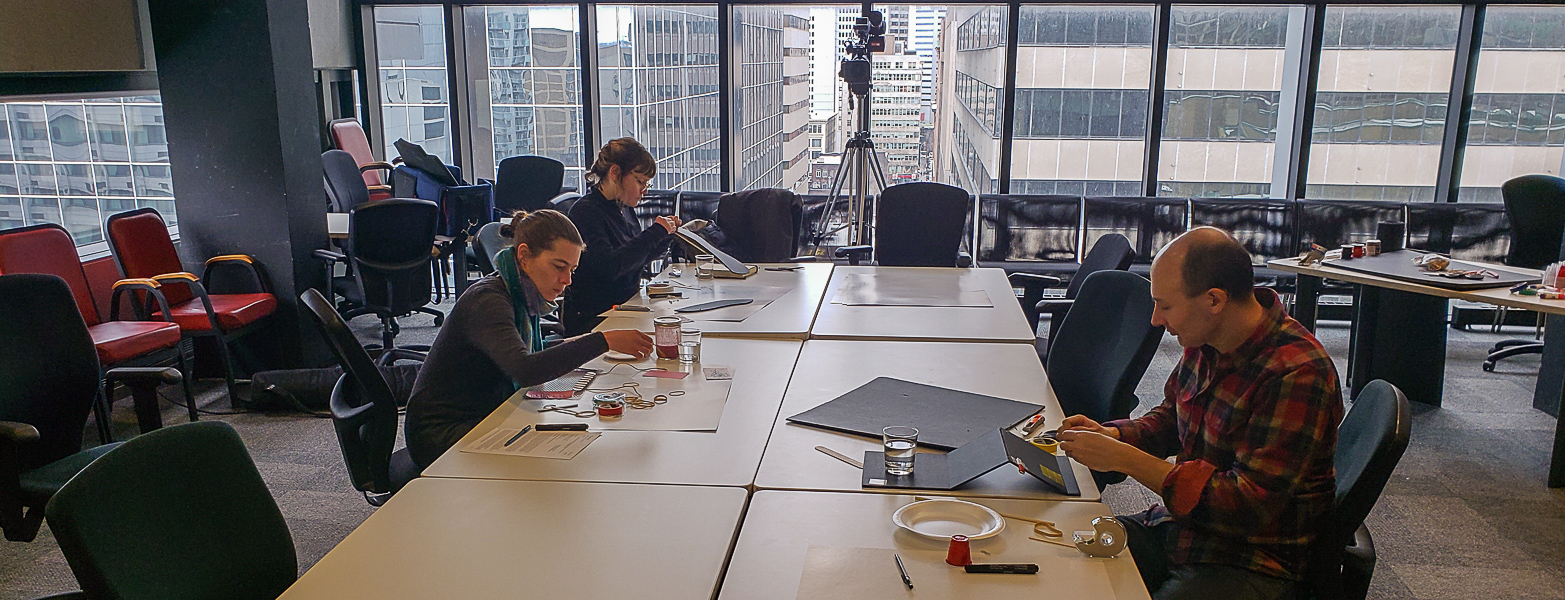
\includegraphics[width=1\textwidth]{ch3_dfp_nfp_A.jpg}
        \caption{Session A.}
        % \label{ch3-fig:keybox-cad}
    \end{subfigure}
    \par\bigskip
    \begin{subfigure}[]{0.59\textwidth}
        \centering
        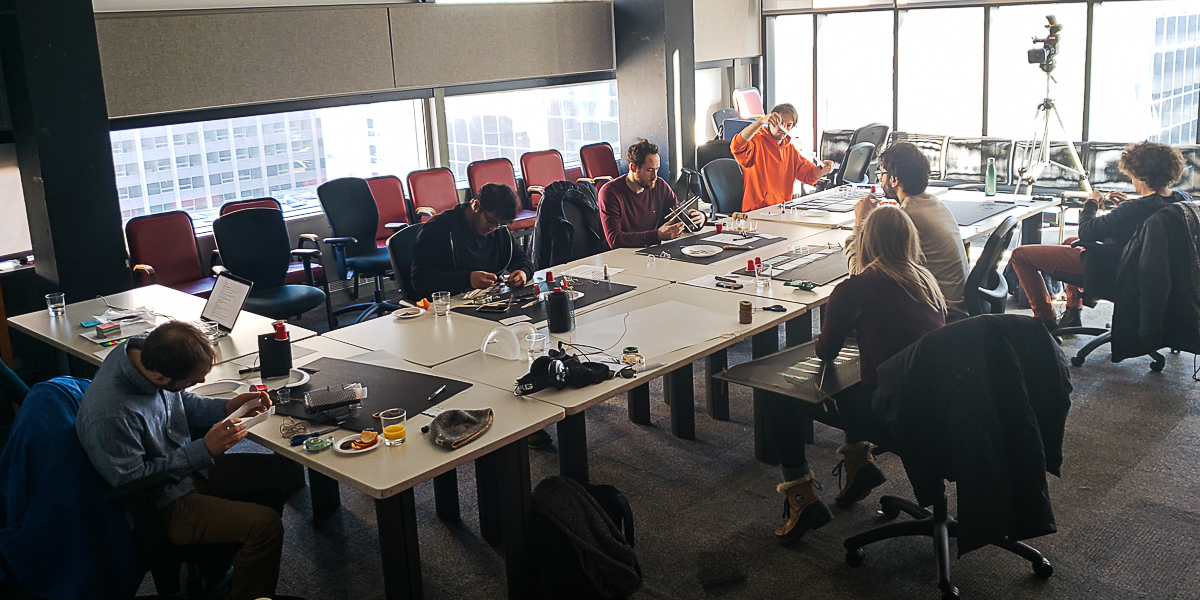
\includegraphics[width=1\textwidth]{ch3_dfp_nfp_B.jpg}
        \caption{Session B.}
        % \label{ch3-fig:stringbox-cad}
    \end{subfigure}
    \begin{subfigure}[]{0.4\textwidth}
        \centering
        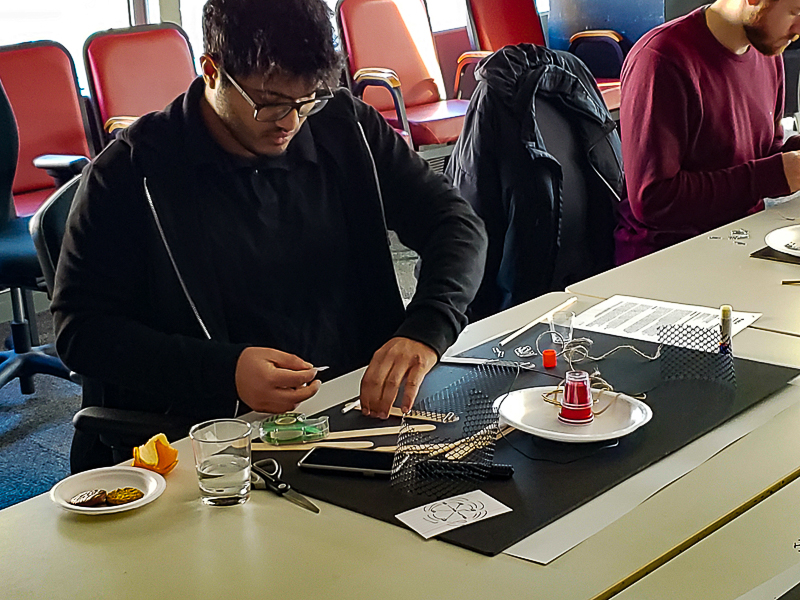
\includegraphics[width=1\textwidth]{ch3_dfp_nfp_B_P4.jpg}
        \caption{Participant P04 in Session B.}
        % \label{ch3-fig:tapbox-cad}
    \end{subfigure}
    \caption[Design for Performance workshop: Activity 2 - Non-functional prototyping]{Participants crafting non-functional instrument prototypes in Activity 2.}
    \label{ch3-fig:instrument-building}
\end{figure}

% The following instructions were given to introduce the activity:

% \begin{itemize}[noitemsep]
%     \item Using the provided materials, you are asked to build an instrument with which you could play the music that you drew.
%     \item Bear in mind that you are building \emph{non-functional} prototypes. Your instruments do not need to sound and, specifically, you should not select or utilize materials for their acoustic properties, nor should you be concerned with technical feasibility. 
% \end{itemize}

To assist the participants in developing their ideas into tangible designs, we introduced an informal list of eight considerations to refer to while building their instruments, which were written on a large whiteboard. The considerations are divided into \emph{high-level} operational qualities and general characteristics that could describe the instrument's intended use (\emph{functionality}, \emph{playability}, \emph{musicality}, \emph{performance context}), and \emph{low-level} essential features and fundamental components of the design (\emph{physical form and ergonomics}, \emph{interaction methods}, \emph{sound production}, \emph{feedback}).

% \begin{itemize}[noitemsep]
%     \item \textbf{Operational qualities:} \emph{functionality}, \emph{playability}, \emph{musicality}, \emph{performance context}. 
%     \item \textbf{Design features and fundamental components:} \emph{physical form and ergonomics}, \emph{interaction methods}, \emph{sound production}, \emph{feedback}
% \end{itemize}

While some of the considerations can be classified as functional and non-functional requirements (as defined by requirements engineering \citep{Glinz2007} and commonly employed in systems design), it is important to point out that these elements were empirically chosen based on our own prior knowledge and experience in DMI design, and left open-ended to provide helpful points of reference through the activity. 
% The considerations were presented along with their descriptions before the activity began, then written on a large whiteboard while the participants worked.

% \begin{table}[htbp]
%     \caption{Design considerations given for non-functional prototyping activity.}
%     \begin{center}
%         \begin{tabular}{L{3cm} L{3cm} L{9cm} }
%             % \hline % \toprule
% \hline
%             \textbf{Category} & \textbf{Consideration} & \textbf{Description} \\
%             % \hline % \midrule
% \hline
%             \multirow{4}{3cm}{Operational qualities and usage} 
%             & Functionality 
%             & How does the instrument function? 
%             \\ 
%             \vspace{0.75em}
%             & Playability 
%             & How do you play it? 
%             \\
%             \vspace{0.75em}
%             & Musicality 
%             & What does it sound like, and how does it facilitate musicality? 
%             \\
%             \vspace{0.75em}
%             & Context 
%             & Where and how will this be used? (types of venues, solo or in groups, etc.)
%             \\ 
%             % \hline % \midrule
% \hline
%             \multirow{4}{3cm}{Design features and fundamental components} 
%             & Physical form and ergonomics
%             & What are the instrument's defining physical characteristics, life size, shape, orientation and posture for the performer?
%             \\
%             \vspace{0.75em}
%             & Interaction methods
%             & What kind of controls and user inputs does it have?
%             \\
%             \vspace{0.75em}
%             & Sound production
%             & How is the sound produced? (ie., synthesis, sampling, live audio processing)
%             \\
%             \vspace{0.75em}
%             & Feedback
%             & What kind(s) of feedback will the instrument provide to the performer?
%             \\  
%             % \hline % \bottomrule
% \hline
%         \end{tabular}
%     \end{center}
%     \label{ch3-tab:design-considerations}
% \end{table}

% The participants were initially given 25 minutes to complete the activity (pictured in Figure \ref{ch3-fig:instrument-building}), though extra time could be allotted if desired. In both sessions, five extra minutes were added, making the total length of the activity 30 minutes. 


\subsubsection{Activity 3: Presentations and key element identification}
\label{ch3-sec:activity-3-presentations}

Following the construction, each participant gave a three minute presentation of their instrument. They began with a description of the music they had drawn, then described and demonstrated their instrument. The participants were encouraged to explain the links between the music on their index cards and the instruments, which helped to orient the presentations on the imagined outcomes rather than the technical details of the fabricated designs. A two minute group discussion followed each presentation. 

While the participants described their instruments the facilitator listened for key elements of their designs, such as essential features, attributes, characteristics that could help to define the instrument. As elements were identified, they were written on sticky notes and posted to the whiteboard, clustered around the eight considerations that had been given in the previous activity. The presenter and other participants were also encouraged to suggest elements which were added to the board. 
% This method of identifying design elements with sticky notes is common in design research \citep{Fischel2018}. The sticky notes were also color coded by participant to allow us to attribute key elements to individual designs \citep{Reichelt2014}, although ultimately a detailed comparative analysis was beyond the scope of this study.

\subsubsection{Activity 4: Dot-voting}
\label{ch3-sec:activity-4-dot-voting}

The key element identification was intended to allow the group collectively to consider aspects of the designs that would be appealing to incorporate into a fully functional instrument. To facilitate this turn, participants were then asked to vote for the elements that they most strongly favored by placing colored stickers (dot votes) next to the items they wished to vote for (as shown in Figure \ref{ch3-fig:dot-voting}). 
% Dot voting is a common activity in design workshops and collaborative sessions to collaboratively prioritize items from a large set \citep{Gibbons2019} and focus attention for discussion and decision making \citep{Gray2010}. Each participant is given a number of stickers to place by the items of their choosing. When they are finished, the votes are calculated and presented to the group for further action. 
Drawing from varying recommendations about the appropriate number of votes per participant \citep{Gray2010, Gibbons2019} and considering the number of participants and elements from each session, each participant was allotted 10 votes.

As we will discuss in next section, this exercise was less oriented around ranking of essential design elements and more concerned with facilitating a discussion around individual and shared priorities for bringing a new instrument to life. The voting activity was completed quickly and the workshop moved on to a final discussion.

\begin{figure}[htbp]
    \begin{minipage}{0.49\textwidth}
        \centering
        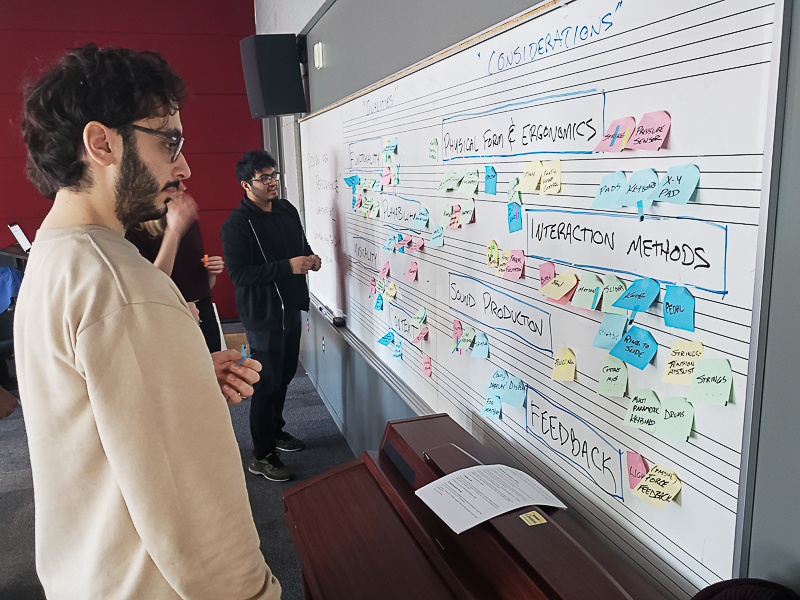
\includegraphics[width=1\textwidth]{ch3_dfp_dot_voting_B.jpg}
        \caption[Design for Performance workshop: Activity 4 - Dot voting]{Session B participants dot voting for essential design elements in Activity 4.}
        \label{ch3-fig:dot-voting}
    \end{minipage}\hfill
    \begin{minipage}{0.49\textwidth}
        \centering
        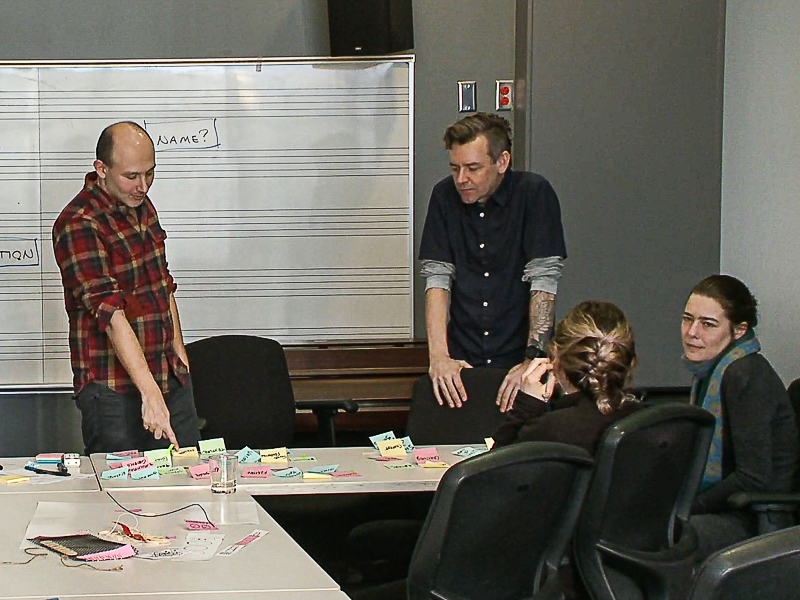
\includegraphics[width=1\textwidth]{ch3_dfp_discussion_A.jpg}
        \caption[Design for Performance workshop: Activity 5 - Discussion]{Session A participants conclude the workshop with a group discussion in Activity 5.}
        \label{ch3-fig:discussion}
    \end{minipage}
\end{figure}

\subsubsection{Activity 5: Group discussion}
\label{ch3-sec:activity-5-group-discussion}

The workshop concluded with a ten minute open discussion (shown in Figure \ref{ch3-fig:discussion}) with the facilitator and participants about the identified key elements and prospects for utilizing them and additional aspects of the instrument designs in the development of new DMIs that they would want to use in their own practice. The facilitator also provided information about future steps for the project including the eventual design of functional instrument prototypes based on the workshop outcomes. The workshop length for session a with three participants; session B, with seven participants, ran longer and was completed in just under two hours. 

\section{Results}
\label{ch3-sec:results}

Workshop results are reported in two parts. First we present the direct outcomes of the workshop activities, then we present results from thematic analysis of the video recorded workshop sessions. 

\subsection{Participant profiles and output}
\label{ch3-sec:participant-profiles-and-output}

In addition to the basic background information collected in the prescreening questionnaire, the self introductions at the beginning of the workshop provided additional insights about the participants' own musical and DMI practices. Profiles of the ten participants are shown in Appendix 1.

In their self-introductions, participants were also asked if they had previous experience with designing digital musical instruments (included in Appendix 1). While this was not a criteria for participation, six of the participants reported at least some previous experience, including P04 and P05 who come from engineering backgrounds and have significant technical knowledge and experience in this area. This is consistent with DMI literature that highlights the overlap between DMI design and practice (see \citet{Magnusson2008, Morreale2017, Morreale2018} for example). While not a specific focus for this study, we can envision a future workshop variant that investigates the differences between designers and non-designers explicitly.

It should be noted that three of the participants were known by the authors. In particular, P09 is an instrumental performer and regular collaborator with the first author. However given the limited size of the local DMI community we determined that this should not disqualify them from participation if they met the defining criteria. 

\subsubsection{Design outputs}
\label{ch3-sec:design-outputs}

During the workshop each participant produced two physical design artefacts: their ``draw the music'' index card (as described in the presentations) and the instruments they designed. The outputs are listed in Appendix 1. To relate the instruments to existing DMI research, the instruments are categorized according to \citeauthor{Miranda2006a}'s classification of gestural controllers (\citeyear{Miranda2006a}): \emph{augmented}, \emph{instrument-like}, \emph{instrument-inspired}, and \emph{alternate}. Given the abstract nature of the ``draw the music'' task and its express purpose to provide an on-ramp and context for the creative activity to follow, it is unnecessary to discuss the output of the cards themselves and instead focus on the instruments that the participants created. 

% \begin{figure}[htbp]
%     \centering
%     \begin{subfigure}{1\textwidth}
%         \centering
%         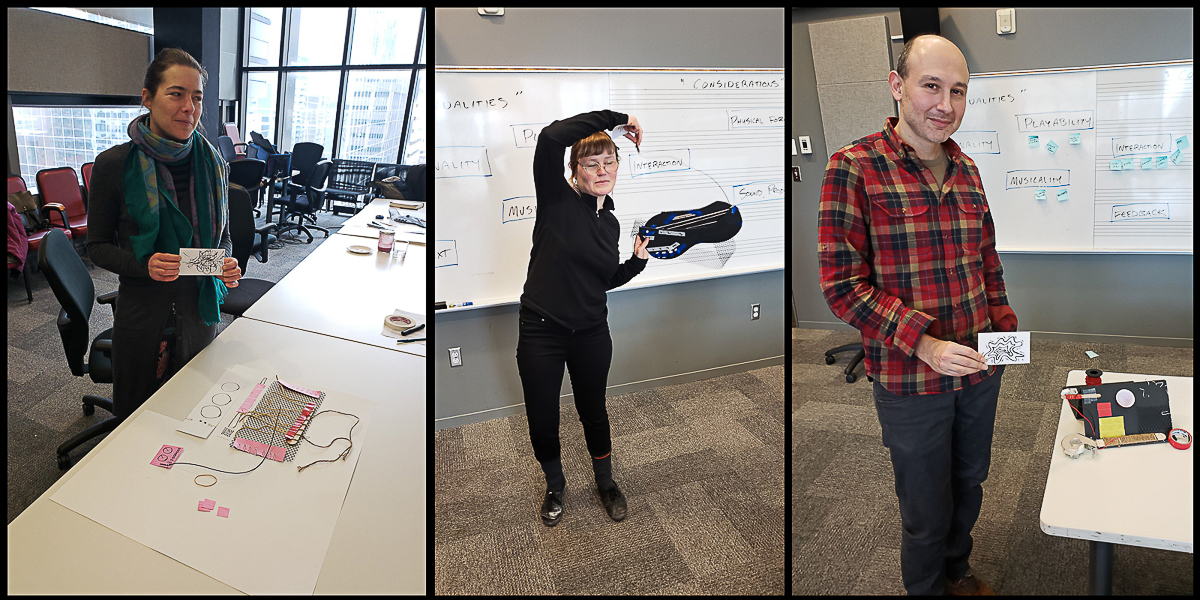
\includegraphics[width=1\textwidth]{ch3_dfp_presentations_A.jpg}
%         \caption{Session A: P01--P03 (left to right)}
%         \label{ch3-fig:presentations_A}
%     \end{subfigure}
%     \par\bigskip
%     \begin{subfigure}{1\textwidth}
%         \centering
%         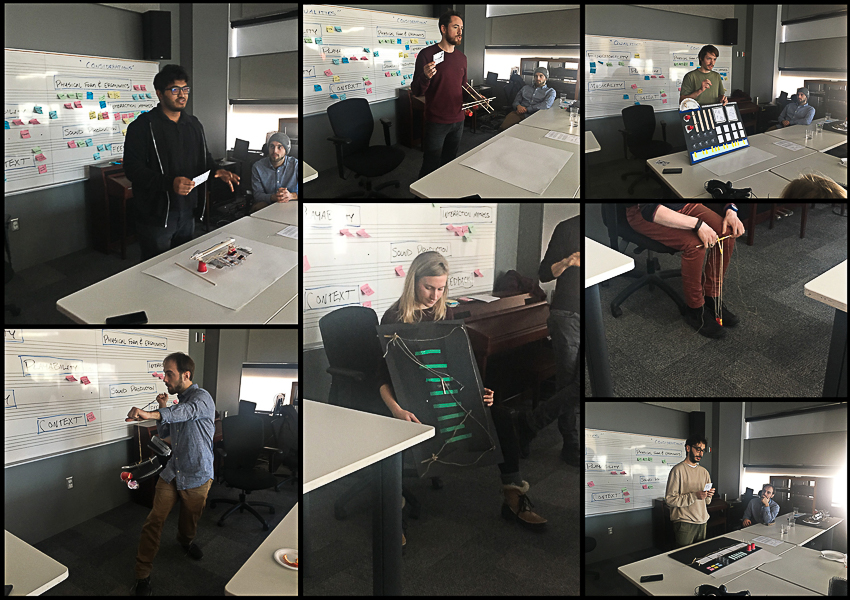
\includegraphics[width=1\textwidth]{ch3_dfp_presentations_B.jpg}
%         \caption{Session B: P04--P10 (clockwise from top left)}
%         \label{ch3-fig:presentations_B}
%     \end{subfigure}
%     \caption[Design for Performance workshop: Activity 3 - Presentations]{Participants present their instrument prototypes in Activity 3.}
%     \label{ch3-fig:presentations}
% \end{figure}


\begin{figure}[htbp]
    \centering
    \begin{subfigure}{0.49\textwidth}
        \centering
        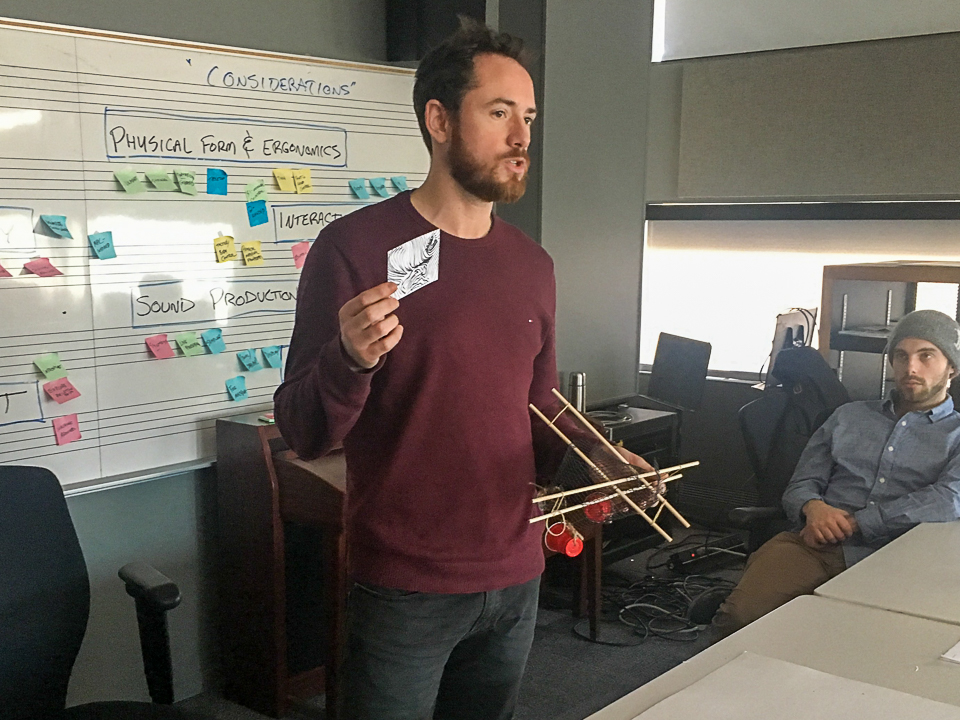
\includegraphics[width=1\textwidth]{CMJ1.jpg}
        \caption{P05}
        \label{ch3-fig:presentations_P05}
    \end{subfigure}
    \begin{subfigure}{0.49\textwidth}
        \centering
        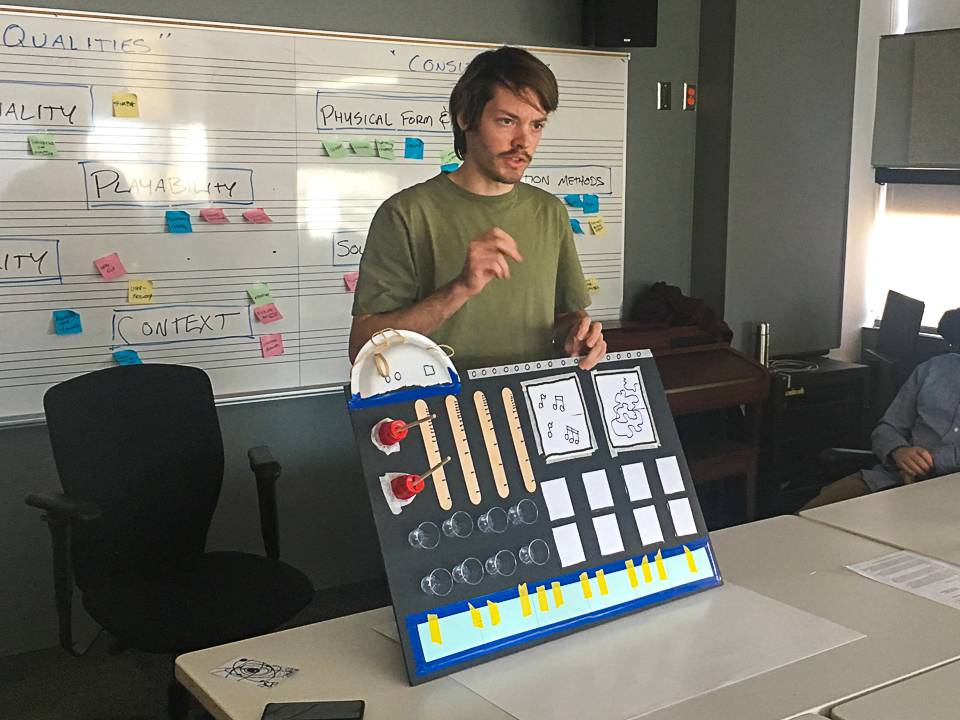
\includegraphics[width=1\textwidth]{CMJ2.jpg}
        \caption{P06}
        \label{ch3-fig:presentations_P06}
    \end{subfigure}
    \begin{subfigure}{0.49\textwidth}
        \centering
        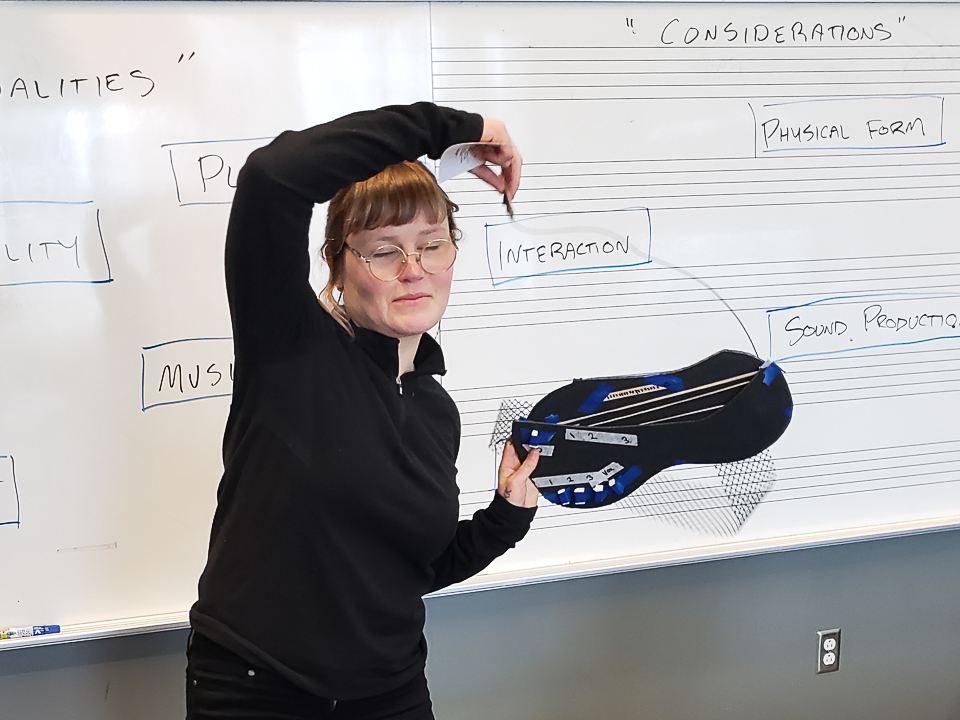
\includegraphics[width=1\textwidth]{CMJ3.jpg}
        \caption{P02}
        \label{ch3-fig:presentations_P02}
    \end{subfigure}
    \begin{subfigure}{0.49\textwidth}
        \centering
        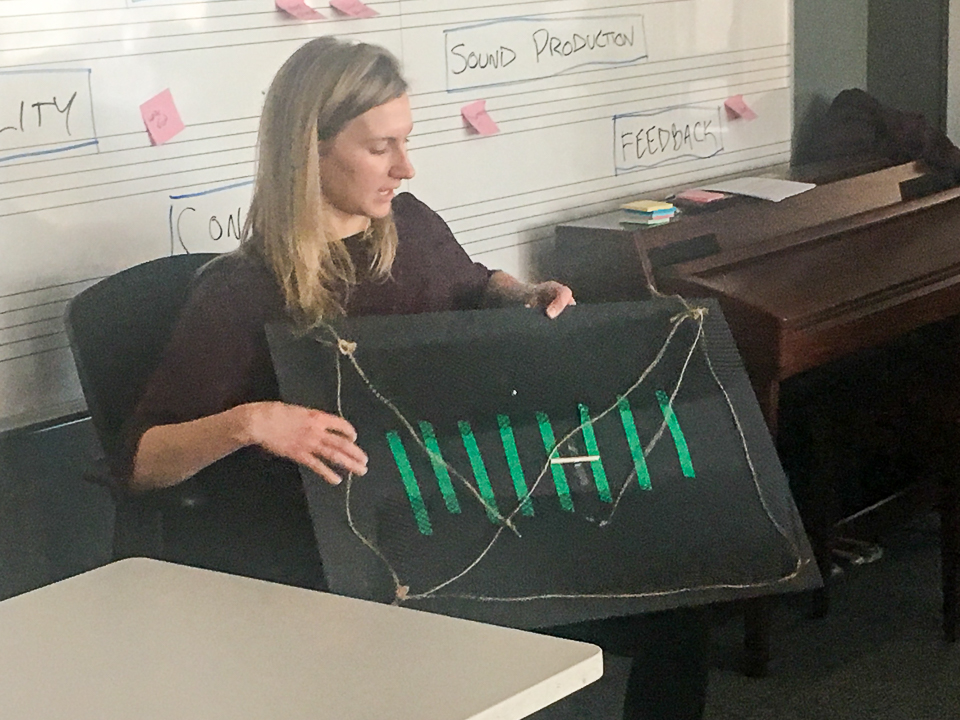
\includegraphics[width=1\textwidth]{CMJ4.jpg}
        \caption{P09}
        \label{ch3-fig:presentations_P09}
    \end{subfigure}
    \caption{Participants present their instrument prototypes in Activity 3.}
    \label{ch3-fig:presentations}
\end{figure}

Half of the instruments can be classified as alternate instruments. While each was entirely unique, the various forms show the strong influence the materials played on the resulting designs, with each instrument prioritizing physical shapes and textures as the focus of the design. For example, P05 created a resonant physical structure built of many different types of materials (Figure \ref{ch3-fig:presentations_P05}). The structure would be excited by touching, tapping, rubbing or plucking different elements, which would generate audio signals to drive multiple different sound processes.

Four of the remaining five instruments can be identified as either instrument-like or instrument-inspired, taking various elements from existing instruments and repurposing them in different ways. A noticeable trend among this group was to combine the functionalities of several instruments into a single instrument, either to be able to play multiple parts simultaneously like P06's multifunction performance workstation (Figure \ref{ch3-fig:presentations_P06}) or to mix them together in creative ways like P02's instrument that would mix and cross-modulate vocals and guitar (Figure \ref{ch3-fig:presentations_P02}). 

There was one augmented instrument designed by P09 (Figure \ref{ch3-fig:presentations_P09}). This participant is an expert instrumentalist with an advanced degree in performance on her instrument, the concert harp. She has been performing electroacoustic music using harp and various external controllers and was clear in her needs and priorities as a performer, which was reflected in the pragmatic approach and practical utility of her design. (As previously mentioned, P09 and the first author are active collaborators whose work is the subject of the following chapter.)

% ...at the time of the workshop P09 and the author the participant and first author had previously collaborated, and would collaborate again, focusing on designing novel technologies for professional performers. 

In Andersen's Magic Machine workshops, the physical objects may serve to evoke inspirations for discussion and conversation within the workshop group, or ``serve as simple vessels for notions and ideas, which are somewhat or completely beyond, what is represented in the model'' \citep[p. 63]{Andersen2017}. This holds true for the Design for Performance workshops as well, and therefore the physical prototypes themselves were not analyzed in further depth. 
% Instead the key element identification and dot-voting activities, followed by the post-workshop thematic analysis of the presentations provided a rich understanding of the participants' designs. 

\subsection{Key elements, dot voting, and discussion}
\label{ch3-sec:key-element-identification-and-dot-voting}

% The remainder of the workshop activities include the key elements compiled during presentations, results and implications of the dot voting activity, and the closing group discussions. 

% In this section, we examine the output of the remaining workshop activities: the key elements compiled during presentations, results and implications of the dot voting activity, and the group discussions that concluded the sessions.

% \subsubsection{Key elements}
% \label{ch3-subsub-key-elements}

As described previously, during the presentations key design elements were identified and posted to the whiteboard. 
% We intentionally refrained from giving a strict definition for what constitutes a ``key element'' in hopes of drawing out intangible aspects of the designs in addition to more obvious and concrete elements. 
% Given the short format of the presentations (three minutes to present and two minutes for discussion), this was not an exhaustive list, however with the active participation of the whole group we attempted to capture most of the essential elements of each instrument. The full list is included in Appendix \ref{axC-sec:key-elements-and-dot-voting-results} showing the elements corresponding to each participant's instrument, as identified from the color-coded sticky notes.  
36 elements were recorded for the three instruments in Session A and 70 elements identified for the seven instruments in Session B, for a total of 106 (averaging 10.6 elements per instrument). As the elements were posted during the presentations, they were clustered around the eight considerations the participants had been given at the start of instrument prototyping exercise . These weren't intended to be strict categorizations and the classification of some elements was ambiguous, but this provided a basic structure that helped to reveal where the attention of the designs was focused. Figure \ref{ch3-fig:key-elements-by-category} shows the distribution of elements across the categories. 

\begin{figure}[htbp]
    \centering
    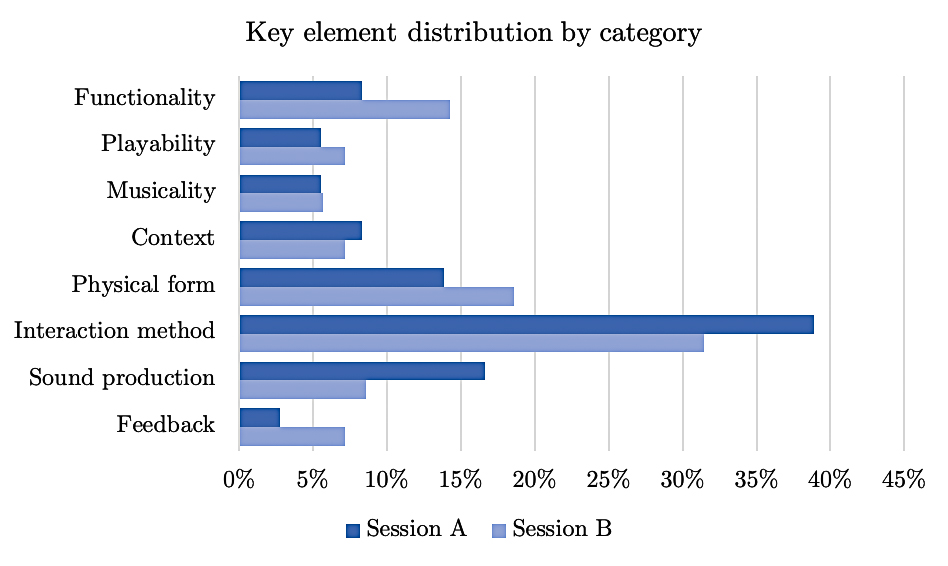
\includegraphics[width=0.75\textwidth]{ch3_key_element_categories}
    \caption[Design for Performance workshop: Key elements by category]{Distribution of key elements by category (design considerations), shown as percentages of total elements identified. For Session A, \emph{N}=36; for Session B, \emph{N}=70.}
    \label{ch3-fig:key-elements-by-category}
\end{figure}

The most common category was \emph{interaction methods}, with roughly one third of all elements related to how the performer would interact with the instrument, naming specific types of controls (like knobs or keys) or describing techniques for playing the instrument (touching, bowing, moving, etc.). While both controls and playing techniques were classified into one category here, it is worthwhile to note that they are not strictly orthogonal. A study by \citep{Marshall2009b} found that musicians tended to use the same control with different interaction techniques and playing strategies. Nonetheless, the frequent mention of both physical controls and instrumental technique highlights the embodied connection between a performer and their instrument that has been a strong theme in DMI research \citep{Emerson2018,Magnusson2007} and third wave HCI \citep{Harrison2007}). On the other hand, the prevalence of this category may also be due in part to the structure and pace of the presentations, where describing these elements (along with physical form, which was the second most frequent category) gave the most succinct description of an instrument in a short time. 

% Another insight from the categorizations is that overall, the more abstract ``operational qualities and usage'' considerations of \emph{functionality}, \emph{playability}, \emph{musicality}, and \emph{context} received far less attention than the more concrete ``design features and fundamental components'' of \emph{physical form}, \emph{interaction methods} and \emph{sound production} (though the fourth category \emph{feedback} was the least identified of all). Again, we refrain from reading too much into this, because the more objective elements may have simply provided the quickest and most direct way to describe the instruments.

% \subsubsection{Dot voting and group discussion}
% \label{ch3-sec:dot-voting-and-group-discussion}

Following the presentations, the participants dot voted for the elements that they would most want to be incorporated into a new instrument design. Table \ref{ch3-tab:dot-voting} shows the top dot voted elements from each session. 

\begin{table}[htbp]
    \centering
    \caption{Top Dot-Voted Key Elements}
    \begin{tabular}{lc|lc}
        \hline
        \multicolumn{2}{c|}{\textbf{\emph{Session A}}} &
        \multicolumn{2}{c}{\textbf{\emph{Session B}}} \\
        % \hline % \toprule
        % \hline
        \textbf{Element} & \textbf{votes} &
        \textbf{Element} & \textbf{votes} \\
        % \hline % \midrule
        \hline
        playful unreliability & 3 & synthesis & 5 \\
        textures & 3 & audiovisual experience & 4 \\
        modular & 3 & pressure sensor & 4 \\
        organic & 2 & plucking & 4 \\
        move while you play & 2 & MIDI output & 3 \\
        blending & 2 & portability & 3 \\
        radio & 2 & strings & 3 \\
        touching & 2 & & \\
        % \hline % \bottomrule
        \hline
    \end{tabular}
    \label{ch3-tab:dot-voting}
    
\end{table}

% In planning the workshop, we imagined the key element identification and dot voting steps could serve two possible functions. First, it could indicate areas of consensus (or disagreement) between the participants' designs that could inform the discussion around prospects of employing elements into functional instruments. Second, we hoped that the process on its own might suggest clear directions to orient our future functional designs. 

In Session A the closing discussion centered around the results of the dot viting. There was a high amount of agreement despite the individual instruments being very different. In particular, the participants valued modular instrument designs that could facilitate mixing and rerouting of signals, and allow the instruments to be flexible for use in a variety of ways. Additionally, the quality of \emph{playful unreliability} was popular, where an instrument might behave in non-deterministic or unexpected ways, leading to novel sounds and new ways of performing. 
% This seemingly runs counter to one of the findings of \citeauthor{Magnusson2007}'s survey (discussed in Chapter \ref{ch2-cha}, Section \ref{ch2-sec:dual-performer-designer-roles}), in which many respondents were intolerant of this quality in digital instruments. However the underlying assumptions aren't necessarily the same. 
This brings to mind Joel Chadabe's description of \emph{interactive composing}, in which the performer ``shares control of the music with the information that is automatically generated by the computer, and that information contains unpredictable elements to which the performer reacts while performing'' \citep[p. 23]{Chadabe1984}. 
% Thus the difference lies in the performer's understanding and expectation of an instrument. If the unreliability is intentional, it can be coopted into their performance; if unintentional, it is more likely viewed as a flawed or malfunctioning instrument. 

In Session B, the discussion was relatively short as the session was nearing the two-hour mark and there was a sense that the participants were ready to leave. In addition, as there were so many elements on the board and a wide variety of elements receiving votes, it was difficult to facilitate a conversation around the distinct elements or specific design ideas. However, a comment by P07 provided a valuable observation:  

\begin{quote}
   \emph{ I'd say that you can sum [an instrument] up with keywords, but sometimes what makes it special or good are all the keywords together. If you take some of the words that were thought by different brains [and put them together in a single instrument], it can turn out like Frankenstein.}
\end{quote}

\section{Thematic analysis}
\label{ch3-sec:thematic-analysis}

The preceding quote elucidates the challenge of moving from the individual and idiosyncratic ideas of the participants (as expert performers and end users), to tangible design specifications that can drive instrument designs. Our intent was for the sessions to serve as a space to freely generate ideas which, as seen in the creativity of the designs, was successful. However a systematic understanding of the participants' designs failed to materialize directly through the element identification and dot voting activities. 
% We can suggest two reasons for this. First, the real time identification of key design elements during the fast-paced presentations may not have captured the full essence of the instruments, especially more nuanced or less pronounced elements, and (as reflected in P07's comment) the connections between them. Second, though not explicitly intended in the workshop design, the ensuing activities (key element identification, voting and discussions) were largely organized in a top down manner, structured around the the eight pre-defined considerations given during the workshop activity. 

To better understand the workshop results, a thematic analysis of the participant presentations was conducted using the methodology presented by \citet{Braun2006}. 
% The goals of the thematic analysis are to organize and describe a data set in rich detail, and the methods are flexible to accommodate a variety of approaches. 
We used an inductive approach, similar to the constant comparison method found in grounded theory \citep{Strauss1994}, in which the data set is coded from the bottom up, and avoids fitting it to any preexisting framework.

Our analysis included the following steps. First, presentations of the ten participants were transcribed from the video recordings. An initial round of open coding was performed on the transcribed presentations, where all codeable incidents were identified and assigned preliminary codes. n a second round of coding the incidents were compared to one another to identify similarities and relationships between them, yielding the final set of codes. The codes were then sorted into themes, which were in turn reviewed and refined, then defined and named. The analysis was conducted using the qualitative data analysis software Nvivo by QSR International. 

% \begin{enumerate}[noitemsep]
%     \item Presentations of the ten participants were transcribed from the video recordings. 
%     \item A round of open coding was performed on the transcribed presentations, where all codeable incidents were identified and assigned preliminary codes. 
%     \item In a second round of coding the incidents were compared to one another to identify similarities and relationships between them, yielding the final set of codes. 
%     \item The codes were then sorted into themes, which were in turn reviewed and refined, then defined and named. 
% \end{enumerate}

% The initial round of open coding was performed using Microsoft Excel, while the rest of the analysis was completed with NVivo\footnote{\url{https://www.qsrinternational.com/nvivo-qualitative-data-analysis-software/}}, qualitative data analysis software. NVivo contains a powerful set of features that are particularly useful to develop a rich understanding and and deep insights out of qualitative data, such as the ability to synchronize video and audio files to text transcripts, and to link the data set to different \emph{nodes} (emerging codes and themes) in a searchable database. This underlying structure made it possible to explore the data from different perspectives throughout the process, which helped us determine our complete list of codes and themes. 

In all, 152 incidents were coded across the ten presentations, yielding 56 individual codes categorized across eleven themes. The full list of codes and themes, along with their mentions by participant, is included in Appendix 2. 

\subsection{Design specifications}
\label{ch3-sec:design-specifications}

To move from open exploration in the workshops to tangible design implementations, we examined the five most common themes (which were mentioned by at least half of the participants) and formulated them into a set of design specifications. In Table~\ref{tab:themes-and-specs}, we list each theme with a description, exemplar quote, and resulting design specification. 

\begin{table}[t]
    \footnotesize
    \centering
    \caption{Analysis Themes, Participant Quotes, and Design Specifications}
    \begin{tabular}{L{0.38\textwidth} L{0.28\textwidth} L{0.26\textwidth}}
        % \hline % \toprule
        \hline
        \textbf{Description} &
        \textbf{Quote} &
        \textbf{Specification} \\
        \hline
        \multicolumn{3}{l}{\textbf{\emph{Interaction styles and input control}}} \\
        Embodied physicality; materials, shapes and textures for unique tactile interactions; strings, movement and position sensing, as well as standard input controls. & 
        ``I bring in different types of textures that you can touch. Touching is an important part of it.'' (P03) & 
        Combine conventional and novel interface elements that prioritize embodied, physical, and material-oriented interactions. \\
        \hline
        
        \multicolumn{3}{l}{\textbf{\emph{Signals, connections, and mapping}}} \\
        Flexible, user-definable signal routing and input mapping; Eurorack-style patching, touchscreen and hardware signal matrixes, configurable wireless networks. &
        ``There could be some kind of tactile matrix that you could change to get different sensors.'' (P01) &
        The instrument should feature flexible audio and control signal routing and mappings. \\
        \hline
        
        \multicolumn{3}{l}{\textbf{\emph{Sound production and processing}}} \\
        Sampling, mixing, and layering sounds; processing external audio; synthesizing and modulating audio signals; exciting resonant acoustic objects for signal generation. &
        ``The idea is to get a physical structure that is resonant by itself \ldots then just one stroke, one gate, propagates one signal all over the other instruments.'' (P05) &
        Generate sound via external audio input and resonant acoustic features; sample, synthesize, mix, modulate and process audio signals. \\
        \hline
        
        \multicolumn{3}{l}{\textbf{\emph{Extending (or inspired by) existing instruments}}} \\
        Referencing specific features, functions and playing styles of other instruments. &
        ``This is like the poor man's version of [the Ondes Martinot], in that the original instrument is really impractical and it's really weird and old technology.'' (P08) &
        Mix familiar elements of existing instruments with novel methods of interaction and sound production. \\
        \hline
        
        \multicolumn{3}{l}{\textbf{\emph{Versatility}}} \\
        Versatile, multipurpose instruments that can be used in different ways and contexts; multifunction controls and interchangeable modules. &
        "I wanted something that makes singing, while playing guitar, while doing lots of stuff to your voice, plus your guitar, easier." (P02) &
        The instrument should feature multiple modes or modules of operation that allow for a variety of playing styles. \\
        \hline
        
        % \multicolumn{3}{l}{\textbf{\emph{Performance environment}}} \\
        % Large-scale performance environments, audiovisual elements, video projections, immersive spaces and audience interaction. &
        % ``So I am imagining I'm playing in a dome-like structure, with the world map projected on to it.'' (P04) &
        % \emph{none} \\
        % \hline
    \end{tabular}
    \label{tab:themes-and-specs}
\end{table}

% No design specification was formulated for the \emph{performance environment} theme. As we will discuss the following section, the specifications would be applied to the design of instruments using an existing instrument framework, which carries its own set of constraints especially in terms of size, available materials and fabrication methods. While the design of large-scale audiovisual environments was appealing to several workshop participants and offers possibilities for future designs, it is beyond the practical scope of our current project. 

\section{Discussion}
\label{ch3-sec:discussion}

The Design for Performance workshops were developed as a strategy to generate novel ideas for new DMIs, using methods from contemporary HCI and participatory design, which prioritize qualitative and situated approaches to design and evaluation. By bringing in expert musicians, we aimed to leverage their tacit knowledge and experience of real-world performance practice in hopes that their input could direct the design of instruments that would be appealing and viable to be taken up into musical practice. The choice to use of design fiction as a primary methodology was made for two reasons. First, by removing technological constraints and considerations, the participants were allowed to freely build non-functional prototypes with a focus on their musical practice, without worrying about the feasibility of implementing their designs into functional instruments. Second, the prompt and instrument building activities situated the participants and designs in a fictional narrative of their own imagining. The playful aspect of the activities urged the participants to be creative and unconventional in their endeavors. 

From a designer's point of view, this approach to capturing ideas generated by musicians, especially those that are highly creative and not bounded by the limitations of technical feasibility, can help to stave off potential creative paralysis, bringing in fresh ideas and a better understanding of priorities for performance.

A large part of the methodology designed for this project was adopted from Andersen's Magic Machine workshop playbook. Regarding the prospects for these methods to be used by other researchers, \citeauthor{Andersen2019} propose that ``the multiplicity of highly personal and interpretive content might serve as an additional and complementary resource to design and HCI workshops, which can then in turn be analyzed, annotated or simply challenge designers'' \citeyear[p. 12]{Andersen2019}. Our work here aims to apply the unique and imaginative approach of of design fiction to collaborate with expert musicians to generate creative new ideas and elements for the design of new instruments. 

% HCI has informed several well-structured approaches to DMI design, which were reviewed in teh Background section. With the Design for Performance workshops we aim to align our methods with current and emerging HCI concerns, especially focusing on embodied interaction, phenomenology and qualitative methods of analysis. We find this approach to be complementary to trends in musical interface design which may combine formal engineering and technical know-how with creative practice, and where the lines between functional design and musical composition may become blurred. 

The path from idea generation to the creation of functional playable instruments is similar to \citeauthor{Calegario2019}'s Probatio \citeyearpar{Calegario2019}, in which an entire design cycle is formed. For Probatio this is achieved in a rapid succession, often in a single workshop session where ideas can be generated and directly explored in hardware, which allows for instant testing and evaluation, and rapid iteration. For this project, we envision the similar progression, but occurring on a longer time frame (including the Design for Performance workshop and subsequent instrument designs), and generating high fidelity prototypes that ultimately can be suitable for use in artistic practice. 

The Design for Performance workshop is intended to be one element of a larger design ecosystem. We envision an iterative design sequence in which multiple workshops can be held to evaluate and refine the resulting instrument designs, similar to the method employed by \citet{Absar2015}, where a sequence of three panels iterated on the development of auditory feedback to assist navigation of a visual information system. An iterative process like this could also employ the Probatio toolkit as a step in the design cycle: Ideas generated from the non-functional prototype designs could be explored in low-fidelity functional models with the Probatio hardware before moving towards the design of high-fidelity prototypes that would be viable for real world use.

\subsection{Limitations and future work}
\label{ch3-sec:limitations-and-future-work}

% \subsubsection{COVID-19 and the ongoing suspension of in-person research }

In our own work we have applied the design specifications that were generated from the workshop to the development of three new DMIs, which are intended to embody several of the aspects that emerged from the participants' designs \cite{Sullivan2020nime}. Additional workshops were planned to present the prototypes back to the participants for evaluation and feedback, however due to disruptions caused by COVID-19 they were postponed indefinitely. While COVID-19 continues to be a serious and ongoing situation around the world, we remain optimistic that it will be brought under control in due time. As such, while it is disruptive to our immediate applied research plans, we look forward to continuing our design research in-person with participants when it is safe. 

% Additionally, there are a variety of tools and methods available to conduct DMI workshops and evaluations remotely through videoconferencing and asynchronous activities (such as recording and uploading practice sessions). However, this requires a thorough evaluation of potential methods and ramifications of this approach, and is not planned for this particular project. 

% \subsubsection{General vs. individual users}
\subsubsection{Generic vs. idiosyncratic design}
\label{ch3-sec:generic-vs-idiosyncratic-design}

The comment by P07 in the closing workshop discussion brings to mind the idea of specificity in design. The participants each created an instrument that was personalized for their own needs and practice, and by combining elements of several different instruments into a single design (the Frankenstein instrument), the essence of any single one may be lost. 

On one hand, we are motivated to orient our designs to address areas of concern for general performers. Our analysis of the workshop designs and presentations showed many design elements that were shared by several of the participants. This presents the opportunity to design instruments that could be used by different performers across different contexts, possibly improving an instrument's chance for long-term and widespread adoption. On the other hand, P07's comment speaks to the idiosyncrasy that characterizes field of DMI design, especially where design and performance roles commonly overlap. 

While this issue is not covered in depth here, our continued work explores both angles, first through the instruments developed from the workshops intended for nonspecific DMI performers \citep{Sullivan2020nime}, and through focused collaborations with individual artists and groups, such as the work with P09 \citep{Sullivan2018}. 

\subsection{Conclusion}
\label{ch3-sec:conclusion}

Here we have reported on a novel approach to generate ideas for the design of new DMIs based on design workshops that employ design fiction, allowing workshop participants to freely imagine and craft non-functional instrument prototypes. The workshop design has adapted from Andersen's Magic Machine Workshops ~\citep{Andersen2017} and is informed by theories for DMI development based on previous design frameworks and HCI literature. 
% In particular the approach emphasizes the tacit knowledge of the participants, in our case, expert musicians, towards the development of new instruments that would be appealing for performers to take up into real-world use. 
% We began by reviewing previous research around DMI design, including motivations for the design and use of new instruments, and various design frameworks that have been proposed. Then we introduced the Design for Performance workshop, which we ran with 10 participants divided into two sessions. 
Analysis of the workshop sessions showed several areas of agreement and preference among the participants, which served as the foundations for a list of design specifications for instruments that performers would be likely to use in their practice. In addition to informing our own new designs, the specifications may be useful to other DMI designers as well. 

% As a continuation to this project (which is presented in Chapter \ref{ch4-cha}), we have applied these specifications to the design of three new instruments that are intended to embody many of the desirable aspects presented by the workshop participants. We also envision future workshops, not only to design new instruments, but also to present our current and ongoing designs for feedback and continued iteration. 

Finally, we also present this research as a methodological contribution of a unique and creative approach to early design stages of idea generation and non-functional prototyping that can serve as the initial steps towards the development of high quality, functional and finished prototypes. These methods, while developed for DMI design, are appropriate for a wide range of applications with within and beyond the creative arts. 


%%%%%%%%%% END OF MAIN TEXT %%%%%%%%%%%%%%%%%


%References
\bibliographystyle{cmj}
\bibliography{diss_bib}

\section*{Appendix 1: Participant profiles and design outputs}

\noindent The following tables present the profiles and design outputs of the workshop participants. Workshop Participant Profiles are compiled from responses to the prescreening questionnaire as well as the self introductions at the beginning of each session. The Workshop Design Outputs are taken from the participants' presentations.

\begin{spacing}{1.1}
    \footnotesize
    \begin{longtable}{ C{0.6cm} C{1.1cm} C{1.3cm} C{1.3cm} C{1.3cm} L{3.2cm} L{4.6cm} }
        \caption*{Workshop Participant Profiles} \\
        
        \hline 
        \textbf{ID} &
        \textbf{Years experience} &
        \textbf{Performances / year} &
        \textbf{Use DMIs} &
        \textbf{Design DMIs} &
        \textbf{Instruments played} &
        \textbf{Musical style and description of practice} \\
        % \hline % \midrule
        \hline

        \multicolumn{6}{l}{ \textbf{Session A}} \\ % \hline % \midrule
        \hline
        
        P01 &
        14 &
        21-50 &
        Always &
        some &
        synths, radios, DIY instruments &
        experimental improvisation; transmission-based, in situ solo and group performance \\ \hline
        
        P02 &
        23 &
        21-50 &
        Rarely &
        no &
        vocals, guitar, synthesizers &
        rock, noise, drone, free improvisation \\ \hline
        
        P03 &
        30 &
        5-20 &
        Often &
        no &
        guitar, piano, keys, modular synth, misc. electronics, other stringed   instruments &
        Electronic, World music, Experimental, Brazilian; sound and FX for film \\ % \hline % \midrule
        \hline
        
        % \multicolumn{6}{|l|}{\rule{0pt}{4ex} \normalsize \textbf{Session B}} \\ \hline
        \multicolumn{6}{l}{ \textbf{Session B} } \\ % \hline % \midrule
        \hline
        
        P04 &
        18 &
        5-20 &
        Often &
        yes &
        piano, guitar, drums, T-stick and Sponge (DMIs) &
        Classical, orchestral, prog rock, metal and blues; more recently into electronic music \\ \hline
        
        P05 &
        20 &
        5-20 &
        Always &
        yes &
        synths, vocals, guitar, DIY instruments &
        Electronic, experimental, pop \\ \hline
        
        P06 &
        13 &
        5-20 &
        Always &
        some &
        sampler, synths &
        Electronic, ambient improvisation; typically plays house parties and dive bars; beat-making (electronic/hip-hop) \\ \hline
        
        P07 &
        10 &
        21-50 &
        Always &
        no &
        guitar, bass, controllers, laptop, Max (software) &
        Contemporary music, noise, electronic; composer \\ \hline
        
        P08 &
        16 &
        5-20 &
        Always &
        some &
        drums, guitar, bass, vocals, piano, laptop, controllers, Ableton Live and Max (software) &
        live electronic music mixed with real instruments: ``Think Radiohead.'' \\ \hline
        
        P09 &
        16 &
        21-50 &
        Often &
        no &
        harp, augmented harp, vocals, laptop, controllers, Ableton Live &
        classical, contemporary, electro-acoustic, free improvisation \\ \hline
        
        P10 &
        17 &
        5-20 &
        Often &
        yes &
        vocals, guitar, harmonica, Myo (biosignal/motion controller), DIY instruments &
        Ska, folk and electroacoustic; incorporates movement, martial arts and theatre performance \\ \hline
        % 1 & 2 & 3 & 4 & 5 & 6 & 7 \\
    \end{longtable}
\end{spacing}

\begin{spacing}{1.1}
    \footnotesize
    \begin{longtable}{ c L{5.5cm} L{6.3cm} C{2.5cm} }
        \caption*{Workshop Design Outputs} \\
        % \hline % \toprule
        \hline
        \textbf{ID} &
        \textbf{``Draw the music'' description} &
        \textbf{Instrument presentation} &
        \textbf{Instrument classification} \\
        % \hline % \midrule
        \hline
        
        \multicolumn{4}{l}{\textbf{Session A}} \\ % \hline % \midrule
        \hline
        
        P01 &
        gestures and organic aspects & 
        modular combination of different sensor inputs that could be mapped and remapped in realtime & 
        alternate instrument \\ \hline
        
        P02 &
        many layers of textures: ``shifting sands of many different sounds [and] melodic lines'' &
        a device for FX processing and cross modulating vocals and guitar &
        instrument-like \\ \hline
        
        P03 &
        layers and textures, slowly going from soft to more powerful &
        a collection of different types of sensors for the performer to interact with sound in many different tactile ways &
        alternate instrument \\ 
        
        % \hline % \midrule
        \hline
        \multicolumn{4}{l}{\textbf{Session B}} \\
        % \hline % \midrule
        \hline
        
        P04 &
        audiovisual performance of multicultural music inside a 360\textdegree \hspace{1em} dome representing the world &
        digital/acoustic hybrid acoustic instrument with features of traditional world instruments &
        instrument-inspired \\ \hline
        
        P05 &
        representation of sound propagating through the air, similar to Chiladny plates \citep{Rossing1982} &
        resonant physical structure to excite many different sound processes &
        alternate instrument \\ \hline
        
        P06 &
        circles and orbits, improvising drones and long and short samples shifting over time &
        multifunction workstation: sampler, sequencer, piano keyboard, dual displays &
        instrument-inspired \\ \hline
        
        P07 &
        drops in the water, ripples moving outwards and overlapping &
        stringed instrument held with feet; strings stretched, pulled, plucked, and manipulated &
        alternate instrument \\ \hline
        
        P08 &
        ``any time I hear or feel sound'', music coming from inside body &
        Ondes-Martinot inspired MIDI controller (ring-continuous control) &
        instrument-inspired \\ \hline
        
        P09 &
        harp strings, sound source that is distributed into a living system &
        interface to augment a harp. indirect acquisition of harp sound and manipulation &
        augmented instrument \\ \hline
        
        P10 &
        vertical layers: low basses, middle light and fast, high clear like clouds &
        hyperactive, need to move, two objects tethered to swing around like nunchucks. &
        alternate instrument \\ 
        % \hline % \bottomrule
        \hline
    \end{longtable}
\end{spacing}

% \section*{Appendix 1: Participant profiles and design outputs}
\section{Appendix 2: Thematic Analysis Codebook}

\noindent The following table shows the codes generated from our thematic analysis of the instrument presentations. They are grouped into themes and are sorted by the number of unique cases (participants) each occurs in. The `Refs' column indicates the total number of times (references) that code appeared, though it may have been mentioned several time by a single participant. Thus we find the `Cases' column to be more accurate, which indicates the number of participants attributed to that element. 

\vspace{3ex}

\begin{spacing}{1.1}
    \footnotesize
    % \topcaption*{Workshop Analysis Codebook}
    \tablefirsthead{%
    \hline
    \textbf{Themes and Codes} & \textbf{Cases} & \textbf{P1} & \textbf{P2} & \textbf{P3} & \textbf{P4} & \textbf{P5} & \textbf{P6} & \textbf{P7} & \textbf{P8} & \textbf{P9} & \textbf{P10} & \textbf{Refs} \\ 
    \hline}
    \tablehead{%
    \hline
    \textbf{Themes and Codes} & \textbf{Cases} & \textbf{P1} & \textbf{P2} & \textbf{P3} & \textbf{P4} & \textbf{P5} & \textbf{P6} & \textbf{P7} & \textbf{P8} & \textbf{P9} & \textbf{P10} & \textbf{Refs} \\ 
    \hline}
    \begin{supertabular}{L{5.3cm}cccccccccccc}
        \emph{\textbf{interaction}} & \emph{\textbf{10}} & \emph{\textbf{X}} & \emph{\textbf{X}} & \emph{\textbf{X}} & \emph{\textbf{X}} & \emph{\textbf{X}} & \emph{\textbf{X}} & \emph{\textbf{X}} & \emph{\textbf{X}} & \emph{\textbf{X}} & \emph{\textbf{X}} & \emph{\textbf{71}} \\
        standard input controls          & 8  & X & X & X &   & X & X &   & X & X & X & 20 \\
        strings                          & 5  &   & X &   & X &   &   & X & X &   & X & 8  \\
        tactile interaction              & 4  & X &   & X &   & X &   & X &   &   &   & 9  \\
        movement and position sensing    & 4  &   & X &   & X &   &   &   &   & X & X & 5  \\
        physical interaction             & 3  &   &   & X &   & X &   & X &   &   &   & 13 \\
        materiality                      & 3  & X &   & X &   & X &   &   &   &   &   & 4  \\
        bowing                           & 3  &   &   & X & X &   &   & X &   &   &   & 3  \\
        continuous control               & 2  &   &   &   & X &   &   &   & X &   &   & 6  \\
        microphone input                 & 2  &   &   &   & X &   &   & X &   &   &   & 2  \\
        bi-manual control                & 1  &   &   &   &   &   &   &   &   & X &   & 1  \\
        \hline

        \emph{\textbf{signals, connections and mapping}} & \emph{\textbf{9}} & \emph{\textbf{X}} & \emph{\textbf{X}} & \emph{\textbf{X}} & \emph{\textbf{X}} & \emph{\textbf{X}} & \emph{\textbf{X}} & & \emph{\textbf{X}} & \emph{\textbf{X}} & \emph{\textbf{X}} & \emph{\textbf{20}} \\
        mapping                          & 8  & X & X & X & X & X & X &   &   & X & X & 15 \\
        control signals \emph{(MIDI, CV, wireless)} & 4  & X &   &   &   & X &   &   & X &   & X & 5  \\ 
        computer                         & 2  &   &   &   &   &   &   &   & X &   & X & 2  \\
        \hline
        \emph{\textbf{sound production and processing}} & \emph{\textbf{9}} & \emph{\textbf{X}} & \emph{\textbf{X}}    & \emph{\textbf{X}} & \emph{\textbf{X}} & \emph{\textbf{X}} & \emph{\textbf    {X}} & \emph{\textbf{X}} & \emph{\textbf{X}} & \emph{\textbf{X}} & & \emph  {\textbf{42}} \\
        external input                   & 6  & X & X & X & X &   & X &   &   & X &   & 8  \\
        mixing sounds                    & 4  &   & X & X & X &   &   &   & X &   &   & 8  \\
        effects                          & 3  &   & X &   &   &   &   & X &   & X &   & 7  \\
        acoustic sound production        & 3  &   &   & X & X & X &   &   &   &   &   & 6  \\
        resonance                        & 3  &   &   & X & X & X &   &   &   &   &   & 5  \\
        sampling                         & 2  &   &   & X &   &   & X &   &   &   &   & 5  \\
        designing own sounds             & 1  &   &   &   &   &   &   &   & X &   &   & 1  \\
        spatialization                   & 1  &   &   &   & X &   &   &   &   &   &   & 1  \\
        synthesized sounds               & 1  &   &   &   & X &   &   &   &   &   &   & 1  \\
        \hline
        
        \emph{\textbf{referencing existing instruments}} & \emph{\textbf{7}} & & \emph{\textbf{X}} & \emph{\textbf{X}  } & \emph{\textbf{X}} & & \emph{\textbf{X}} & \emph{\textbf{X}} & \emph   {\textbf{X}} & \emph{\textbf{X}} & & \emph{\textbf{23}} \\
        keyboards and pianos             & 4  &   &   & X & X &   & X &   & X &   &   & 6  \\
        guitar                           & 2  &   & X &   &   &   &   & X &   &   &   & 4  \\
        vocals                           & 2  &   & X &   &   &   &   &   & X &   &   & 4  \\
        Ondes-Martinot                   & 2  &   &   &   &   &   & X &   & X &   &   & 2  \\
        DAW production                   & 1  &   &   &   &   &   & X &   &   &   &   & 2  \\
        augmented instrument             & 1  &   &   &   &   &   &   &   &   & X &   & 1  \\
        drums                            & 1  &   &   &   & X &   &   &   &   &   &   & 1  \\
        harp                             & 1  &   &   &   &   &   &   &   &   & X &   & 1  \\
        instrument-inspired              & 1  &   & X &   &   &   &   &   &   &   &   & 1  \\
        sampler                          & 1  &   &   &   &   &   & X &   &   &   &   & 1  \\
        \hline
    
        \emph{\textbf{versatility}} & \emph{\textbf{6}} & \emph{\textbf{X}} & \emph{\textbf{X}} & & \emph{\textbf{X}} & \emph{\textbf{X}} & \emph{\textbf{X}} & & & & \emph{\textbf{X}} & \emph{\textbf{29}} \\
        combining functions              & 4  & X & X &   & X &   & X &   &   &   &   & 8  \\
        multipurpose/function            & 4  & X &   &   & X & X & X &   &   &   &   & 7  \\
        flexible routing                 & 3  & X &   &   & X &   & X &   &   &   &   & 4  \\
        fungibility                      & 3  & X &   &   &   & X &   &   &   &   & X & 3  \\
        modularity                       & 2  & X &   &   &   & X &   &   &   &   &   & 5  \\
        independent elements             & 1  &   & X &   &   &   &   &   &   &   &   & 2  \\
        \hline
        
        \emph{\textbf{performance environment}} & \emph{\textbf{5}} & & \emph{\textbf{X}} & & \emph{\textbf{X}} & & \emph{\textbf{X}} & & & \emph{\textbf{X}} & \emph{\textbf{X}} & \emph{\textbf{12}} \\
        audiovisual                      & 4  &   &   &   & X &   & X &   &   & X & X & 7  \\
        physical space and movement     & 2  &   & X &   &   &   &   &   &   &   & X & 3  \\
        audience                         & 1  &   &   &   &   &   &   &   &   &   & X & 1  \\
        immersive environment            & 1  &   &   &   & X &   &   &   &   &   &   & 1  \\
        \hline
    
        \emph{\textbf{size and form factor}} & \emph{\textbf{4}} & \emph{\textbf{X}} & \emph{\textbf{X}} & & \emph{\textbf{X}} & & & \emph{\textbf{X}} & & & & \emph{\textbf{10}} \\
        stand-alone embedded             & 4  & X & X &   & X &   &   & X &   &   &   & 5  \\
        portable                         & 1  &   &   &   &   &   &   & X &   &   &   & 2  \\
        radio                            & 1  & X &   &   &   &   &   &   &   &   &   & 2  \\
        large immersive space            & 1  &   &   &   & X &   &   &   &   &   &   & 1  \\
        \hline
    
        \emph{\textbf{desirable or undesirable qualities}} & \emph{\textbf{4}} & & & & & & \emph{\textbf{X}} & \emph{\textbf{X}} & \emph{\textbf{X}} & & \emph{\textbf{X}} & \emph{\textbf{5}} \\
        limitation of current instrument & 2  &   &   &   &   &   & X &   & X &   &   & 2  \\ 
        DIY                              & 1  &   &   &   &   &   &   & X &   &   &   & 1  \\
        simple                           & 1  &   &   &   &   &   &   & X &   &   &   & 1  \\
        stability                        & 1  &   &   &   &   &   &   &   &   &   & X & 1  \\
        \hline
    
        \emph{\textbf{posture}} & \emph{\textbf{3}} & & \emph{\textbf{X}} & & & & & & & \emph{\textbf{X}} & \emph{\textbf{X}} & \emph{\textbf{3}} \\
        sitting                          & 1  &   &   &   &   &   &   &   &   & X &   & 1  \\
        strap                            & 1  &   & X &   &   &   &   &   &   &   &   & 1  \\
        walking                          & 1  &   &   &   &   &   &   &   &   &   & X & 1  \\
        \hline
    
        \emph{\textbf{feedback}} & \emph{\textbf{2}} & & & & & & \emph{\textbf{X}} & \emph{\textbf{X}} &   &   &   & \emph{\textbf{4}}  \\
        visual display                   & 1  &   &   &   &   &   & X &   &   &   &   & 3  \\
        passive haptic feedback          & 1  &   &   &   &   &   &   & X &   &   &   & 1  \\
        \hline

        \emph{\textbf{cultural context}} & \emph{\textbf{1}} & & & & \emph{\textbf{X}} & & & & & & & \emph{\textbf{3}} \\
        geographical and cultural relevance  & 1  &   &   &   & X &   &   &   &   &   &   & 3  \\
        \hline
    \end{supertabular}
\end{spacing}

\end{document}
